\documentclass{article}

\usepackage{blindtext}
\usepackage[utf8]{inputenc}

\usepackage{graphicx,fancyhdr,amsmath,amssymb,amsthm,subfig,url,hyperref}
\usepackage{algorithm}
\usepackage{algpseudocode}
\usepackage{booktabs}
\usepackage{float}
\restylefloat{table}
\usepackage[margin=1in]{geometry}
\usepackage{amsthm}
\usepackage{multirow}
\usepackage{enumitem}
%\usepackage{enumerate}
\usepackage[normalem]{ulem}
\usepackage{accents}
\usepackage{thm-restate}
\usepackage{physics}
\usepackage[numbers]{natbib}

\usepackage{todonotes}

\newcommand{\specialcell}[2][c]{%
  \begin{tabular}[#1]{@{}c@{}}#2\end{tabular}}

%----------------------- Macros and Definitions --------------------------

%%% FILL THIS OUT
\newcommand{\studentname}{Oliver Hinder}
\newcommand{\suid}{ohinder}
%%% END

\newcommand{\ubar}[1]{\underaccent{\bar}{#1}}

 
%\usepackage{algorithm,algcompatible,amssymb,amsmath}

%\renewcommand{\COMMENT}[2][.5\linewidth]{%
%  \leavevmode\hfill\makebox[#1][l]{//~#2}}
%\algnewcommand\algorithmicto{\textbf{to}}
%\algnewcommand\RETURN{\State \textbf{return} }

% If {a} then b End
\algnewcommand{\IfR}[1]{\State\algorithmicif\ #1\ \algorithmicthen}
\algnewcommand{\EndIfR}{\unskip\ \algorithmicend\ \algorithmicif}


\renewcommand{\theenumi}{\bf \Alph{enumi}}

\theoremstyle{plain}
\newtheorem{theorem}{Theorem}
\newtheorem{assumption}{Assumption}
\newtheorem{example}{Example}


\newtheorem{claim}[theorem]{Claim}
\newtheorem{observation}[theorem]{Observation}

\newtheorem{lemma}[theorem]{Lemma}
%\newtheorem{assume}[assume]{Assumption}
%\newtheorem{example}[example]{Example}


\newtheorem{corollary}[theorem]{Corollary}
\newtheorem{definition}[theorem]{Definition}
\newtheorem{remark}[theorem]{Remark}
\newtheorem{fact}[theorem]{Fact}
%\declaretheorem[name=Theorem,numberwithin=section]{thm}
%\declaretheorem[name=Lemma,numberwithin=section]{lem}


\newcommand{\matStart}{\begin{pmatrix}}
\newcommand{\matEnd}{\end{pmatrix}}

\fancypagestyle{plain}{}
\pagestyle{fancy}
\fancyhf{}
\fancyhead[RO,LE]{\sffamily\bfseries\large Stanford University}
\fancyfoot[LO,RE]{\sffamily\bfseries\large \studentname: \suid @stanford.edu}
\fancyfoot[RO,LE]{\sffamily\bfseries\thepage}
\renewcommand{\headrulewidth}{1pt}
\renewcommand{\footrulewidth}{1pt}

\graphicspath{{figures/}}


\def\CompBeta{\beta}

\def\CompBetaAgg{\sigma_{7}}

\def\ArmijoBeta{\sigma_{2}}

\def\ProxResBeta{\sigma_{3}}

\def\BetaSafeAggr{**?**}

\def\BetaSafe{\sigma_{4}}

\def\BetaBacktrack{\sigma_{5}}

\def\BetaVarTheta{\sigma_{6}}

\def\NumCon{m}
\def\NumVar{n}
\def\n{n}
\def\L{L}
\newcommand{\bigO}[1]{O\left( #1 \right)}
\newcommand{\bigSO}[1]{\hat{O}\left( #1 \right)}

\def\R{R}


\def\ResKKT{\mathcal{K}}
\def\ResPrimal{\mathcal{P}}
\def\ResComp{\mathcal{C}}
\def\MeritComp{\mathcal{\zeta}}

\def\T{\mathcal{T}_{\mu}}
\def\Q{\mathcal{Q}_{\mu}}

\def\v{v}

\def\LipP{L_{p}}
\def\LipFun{L_{0}}
\def\LipGrad{L_{1}}
\def\LipHess{L_{2}}
\def\LipCube{L_{3}}

\def\DeltaF{D_{f}}

\def\Diag{\text{Diag}}

\def\X{\mathcal{X}}

\def\Lag{\mathcal{L}}

\def\N{\mathbb{N}}


% ALGORITHMS

\def\AlgTrust{Primal-dual-trust-region}
\newcommand{\callAlgTrust}[1]{\hyperref[AlgTrust]{\Call{\AlgTrust}{#1}}}
\def\AlgMain{non-convex-IPM}
\newcommand{\callAlgMain}[1]{\hyperref[AlgMain]{\Call{\AlgMain}{#1}}}



\usepackage{enumitem}

\begin{document}

\title{A one-phase IPM for non-convex optimization}
\author{Oliver Hinder, Yinyu Ye}

\algdef{SE}[SUBALG]{Indent}{EndIndent}{}{\algorithmicend\ }%
\algtext*{Indent}
\algtext*{EndIndent}

\maketitle


%\def\inProgress{1}
\def\inProgress{0}

\if\inProgress1
\newcommand{\inProgressHide}[1]{#1} % show
\newcommand{\yinyu}[1]{{\color{red} Yinyu: #1}}
\newcommand{\hinder}[1]{{\color{red}{Hinder: #1}}}
\else
\newcommand{\inProgressHide}[1]{} % hide
\newcommand{\yinyu}[1]{}
\newcommand{\hinder}[1]{}
\fi


\newcommand{\kStart}{k_{\text{start}}}
\newcommand{\kEnd}{k_{\text{end}}}

\newcommand{\algorithmicbreak}{\textbf{break}}
\newcommand{\obj}{f}
\newcommand{\cons}{a}
\newcommand{\hess}{\grad^2}
\newcommand{\nvar}{n}
\newcommand{\ncon}{m}

%\renewcommand{\vec}[1]{\mathbf{#1}}
\renewcommand{\vec}[1]{#1}

\newcommand{\eye}{I}
\newcommand{\ones}{\vec{e}}
\newcommand{\dir}[1]{\vec{d}_{\vec{#1}}}
\newcommand{\Dir}[1]{D_{\vec{#1}}}


\newcommand{\LDL}{LDL}
\newcommand{\LBL}{LBL}

%%%%%%%%%%%%%%%%%%%%%%%%%%
%%%%%%%%%%%%%%%%%%%%%%%%%%
%% BEGIN ALG PARS
%%%%%%%%%%%%%%%%%%%%%%%%%%
%%%%%%%%%%%%%%%%%%%%%%%%%%


\newcommand{\parNumCor}{j_{\max}}
\newcommand{\parNumCorValue}{3}


%% beta

%\newcommand{\parRegularizer}{\beta_{1}}
%\newcommand{\parRegularizerValue}{10^{-8}}
%\newcommand{\parRegularizerInterval}{(0,\infty)}

\newcommand{\parConRegularizer}{\beta_{1}}
\newcommand{\parConRegularizerValue}{10^{-4}}
\newcommand{\parConRegularizerInterval}{(0,1)}

\newcommand{\parComp}{\beta_{2}}
\newcommand{\parCompValue}{0.01}
\newcommand{\parCompInterval}{(0,1)}

\newcommand{\parCompAgg}{\beta_{3}}
\newcommand{\parCompAggValue}{0.02}
\newcommand{\parCompAggInterval}{(\parComp,1)}

\newcommand{\parObjReductFactor}{\beta_{4}}
\newcommand{\parObjReductFactorValue}{0.2}
\newcommand{\parObjReductFactorInterval}{(0,1)}

\newcommand{\parMinStableStepSize}{\beta_{5}}
\newcommand{\parMinStableStepSizeValue}{2^{-5}}
\newcommand{\parMinStableStepSizeInterval}{(0,1)}

\newcommand{\parKKTReductFactor}{\beta_{6}}
\newcommand{\parKKTReductFactorValue}{0.01}
\newcommand{\parKKTReductFactorInterval}{(0,1)}

\newcommand{\parBacktracking}{\beta_{7}}
\newcommand{\parBacktrackingValue}{0.5}
\newcommand{\parBacktrackingInterval}{(0,1)}

\newcommand{\parFracBoundaryExp}{\beta_{8}}
\newcommand{\parFracBoundaryExpValue}{1.5}
\newcommand{\parFracBoundaryExpInterval}{(1,2)}

\newcommand{\parFracBoundary}{\Theta^{b}}
\newcommand{\parFracBoundaryValue}{0.1}
\newcommand{\parFracBoundaryInterval}{(0,1)}

\newcommand{\parFracBoundaryMax}{\Theta^{p}}
\newcommand{\parFracBoundaryMaxValueLinear}{0.1}
\newcommand{\parFracBoundaryMaxValueNL}{0.25}
\newcommand{\parFracBoundaryMaxInterval}{[\parFracBoundary_{i,i}, 1)}


\newcommand{\parInitialize}{\beta_{9}}
\newcommand{\parInitializeValue}{10^{-4}}
\newcommand{\parInitializeInterval}{(0,1)}


\newcommand{\minStepFunc}{\omega}

%%%%%%%%%%%%%%%%%%%%%


%\newcommand{\parFilterReduceBarrier}{\beta_{13}}
%\newcommand{\parMaxRatioPrimalMu}{\beta_{14}}

\newcommand{\parDeltaMin}{\Delta_{\min}}
\newcommand{\parDeltaMinValue}{10^{-8}}
\newcommand{\parDeltaMinInterval}{(0,\infty)}

\newcommand{\parDeltaIncreaseFailure}{\Delta_{\text{inc}}}
\newcommand{\parDeltaIncreaseFailureValue}{8}
\newcommand{\parDeltaIncreaseFailureInterval}{(1,\infty)}

\newcommand{\parDeltaDecrease}{\Delta_{\text{dec}}}
\newcommand{\parDeltaDecreaseValue}{3}
\newcommand{\parDeltaDecreaseInterval}{(1,\infty)}


\newcommand{\parDeltaMax}{\Delta_{\max}}
\newcommand{\parDeltaMaxValue}{10^{40}}
\newcommand{\parDeltaMaxInterval}{(\parDeltaMin,\infty)}

\newcommand{\deltaPrev}{\delta_{\text{prev}}}
\newcommand{\parDeltaStart}{\Delta_{\text{start}}}

\newcommand{\parMaxItValue}{3,000}

% tol

\newcommand{\TOLopt}{\epsilon_{\textbf{opt}}}
\newcommand{\TOLoptValue}{10^{-6}}
\newcommand{\TOLoptInterval}{(0,\infty)}

\newcommand{\TOLinf}{\epsilon_{\textbf{inf}}}
\newcommand{\TOLinfValue}{10^{-6}}
\newcommand{\TOLinfInterval}{(0,1)}

\newcommand{\TOLinfOne}{\epsilon_{\textbf{far}}}
\newcommand{\TOLinfOneValue}{10^{-4}}
\newcommand{\TOLinfOneInterval}{(0,1)}

\newcommand{\TOLinfTwo}{\epsilon_{\textbf{inf}}}
\newcommand{\TOLinfTwoValue}{10^{-6}}
\newcommand{\TOLinfTwoInterval}{(0,1)}

\newcommand{\TOLall}{\epsilon}

\newcommand{\infeasFuncOne}{\infeasFunc_{\text{far}}}
\newcommand{\infeasFuncTwo}{\infeasFunc_{\text{inf}}}



\newcommand{\TOLunbounded}{\epsilon_{\textbf{unbd}}}
\newcommand{\TOLunboundedValue}{10^{-8}}
\newcommand{\TOLunboundedInterval}{(0,1)}



%%%%%%%%%%%%%%%%%%%%%%%%%%
%%%%%%%%%%%%%%%%%%%%%%%%%%
%% END ALG PARS
%%%%%%%%%%%%%%%%%%%%%%%%%%
%%%%%%%%%%%%%%%%%%%%%%%%%%




%\newcommand{\Filter}{\mathbb{F}}
\newcommand{\History}{\mathbb{H}}
\newcommand{\conWeight}{\vec{w}}
\newcommand{\ConWeight}{W}
\newcommand{\zeroSet}{Z}
\newcommand{\nonzeroSet}{N}
\newcommand{\alphaMinAgg}{\alpha_{\min}}
\newcommand{\barrier}{\psi}
\newcommand{\regularizer}{r}
\renewcommand{\R}{\mathbb{R}}
\newcommand{\Schur}{\mathcal{M}}
%\newcommand{\Schur}[1]{\mathcal{M}#1}
\newcommand{\MatrixSchur}[2]{\mathcal{H}_{#1}(#2)}


\newcommand{\termination}{\eqref{terminate-kkt}, \eqref{terminate-primal-infeasible} or \eqref{terminate-dual-infeasible}}
\newcommand{\infeasFunc}{\Gamma}


\newcommand{\maxgrad}{G}


\newcommand{\status}{\textbf{status}}
\newcommand{\success}{\textsc{success}}
\newcommand{\failure}{\textsc{failure}}
\newcommand{\maxDelta}{\textsc{max-delta}}


\newcommand{\feasible}{\textbf{feasible}}

\newcommand{\meritKKT}{\mathbb{K}}

\newlength\myindent % define a new length \myindent
\setlength\myindent{6em} % assign the length 2em to \myindet
\newcommand\bindent{%
  \begingroup % starts a group (to keep changes local)
  \setlength{\itemindent}{\myindent} % set itemindent (algorithmic internally uses a list) to the value of \mylength
  \addtolength{\algorithmicindent}{\myindent} % adds \mylength to the default indentation used by algorithmic
}
\newcommand\eindent{\endgroup} % closes a group

% alg
\newcommand{\simpleIPM}{Simplified-One-Phase-Non-Convex-IPM}
\newcommand{\callSimpleIPM}{\Call{Simplified-One-Phase-Non-Convex-IPM}}

\newcommand{\backtrackBlurb}{\emph{Perform a backtracking line search on the primal step $\alpha_{P}$.} Trial step sizes $\alpha_{P} \in \{\alpha^{\max}_{P}, \parBacktracking \alpha^{\max}_{P}, \parBacktracking^2 \alpha^{\max}_{P}, \dots \}$ computing the trial point $(\mu^{+}, x^{+}, s^{+}, y^{+})$ as described in \eqref{eq:primal-iterate-update} and \eqref{eq:alpha-D}. Terminate with $\status = \success$ and return the trial point the first time each of the following conditions hold:}

\begin{center}
\color{red}
\large Draft: Please do not distribute
\end{center}

\begin{abstract}
The work of \citet*{wachter2000failure} suggests that infeasible-start interior point methods (IPMs) developed for linear programming cannot be adapted to nonlinear optimization without significant modification, i.e., using a two-phase or penalty method. We propose an IPM that, by careful initialization and updates of the slack variables, is guaranteed to find a first-order certificate of local infeasibility, local optimality or unboundedness. Our proposed algorithm differs from other IPM methods for non-convex programming because we reduce primal feasibility at the same rate as the barrier parameter. This gives an algorithm with more robust convergence properties and closely resembles successful algorithms from linear programming. We implement the algorithm and compare with IPOPT on a subset of CUTEst problems. Our algorithm requires a similar median number of iterations, but fails on only 9\%  of the problems compared with 16\% for IPOPT. Experiments on infeasible variants of the CUTEst problems indicate superior performance for detecting infeasibility. 
\end{abstract}

\section{Introduction}

\hinder{
To do:
\begin{enumerate}
\item Make implementation consistent with paper (flip signs etc)
\item Replace aggressive term with affine?
\item Explain that Mehrotra's initialization etc is just shifted barrier on the dual
\end{enumerate}
}


Consider the following problem
\begin{subequations}\label{original-problem} 
\begin{flalign}
\min_{x \in \R^{\nvar}}{\obj(x)} \\
\cons(x) \le 0,
\end{flalign}
\end{subequations}
where the functions $a : \R^{\nvar} \rightarrow \R^{\ncon}$ and $f : \R^{\nvar} \rightarrow \R$ are twice differentiable and might be non-convex. Examples of real-world problems in this framework include truss design, robot control, aircraft control, and aircraft design, e.g., the problems TRO11X3, ROBOT, AIRCRAFTA, AVION2 in the CUTEst test set \cite{gould2015cutest}. This paper develops an interior point method for finding KKT points of \eqref{original-problem}, i.e., points such that
\begin{subequations}\label{original-problem} 
\begin{flalign}
\grad \obj(x) - \grad \cons(x)^T y &= 0 \\
y^T \cons(x) &= 0 \\
\cons(x) &\le 0, y \ge 0.
\end{flalign}
\end{subequations}
Interior point methods were first developed by \citet*{karmarkar1984new} for linear programming. The idea for primal-dual interior point methods originates with \citet*{megiddo1989pathways}. Initially, algorithms that required a feasible starting point were studied \cite{kojima1989primal,monteiro1989interior}. However, generally one is not given an initial point that is feasible. A naive solution to this issue is to move the constraints into the objective  by adding a large penalty for constraint violation (Big-M method) \cite{mcshane1989implementation}. A method to avoid the penalty approach, with a strong theoretical foundation for linear programming, is the homogeneous algorithm \cite{andersen1998computational,andersen1999homogeneous,ye1994nl}. This algorithm measures progress in terms of the KKT error, which may not monotonically decrease in the presence of non-convexity\footnote{This occurs even in the one-dimensional unconstrained case, e.g., consider minimizing the function $f(x)=-9 x - 3 x^2 + x^4/4$ starting from zero; the gradient norm increases then decreases.}. It is therefore difficult to generalize the homogeneous algorithm to nonconvex optimization. An alternative to the homogeneous algorithm is the infeasible-start algorithm of Lustig \cite{lustig1990feasibility}, which has fewer numerical issues and a smaller iteration count than the big-M method of \cite{mcshane1989implementation}. This approach also simplifies the algorithm by avoiding the need to make a good initial guess for the size of the penalty parameters. Lustig's approach was further improved in the predictor-corrector algorithm of \citet*{mehrotra1992implementation}. This algorithm reduced complementarity, duality and primal feasibility at the same rate, using an adaptive heuristic. This class of methods was shown by \citet*{todd2003detecting} to converge to optimality or infeasibility certificates (of the primal or dual). 
% before reaching the minimizer and only stationary point at $x = 2$.}
%This infeasible-start algorithm was combined with predictor-corrector technique of Mehrotra \cite{ye1993quadratic} into an algorithm with excellent practical performance. 

The infeasible-start method for linear programming \cite{lustig1990feasibility} naturally extends to nonlinear optimization \cite{kortanek1997infeasible},
and most interior point codes for non-convex optimization are built off these ideas \cite{byrd2006knitro,vanderbei1999loqo,wachter2006implementation}. However, \citet*{wachter2000failure} showed that for the problem
\begin{subequations}\label{failure-ex}
\begin{flalign}
\min { x }\\
x^2 - s_1 - 1 &= 0 \\
x - s_2 - 1/2 &= 0 \\
s_1, s_2 &\ge 0
\end{flalign}
\end{subequations}
a large class of infeasible-start algorithms fails to converge to either a local optimum or infeasibility certificate starting at any point with $x < 0$, $s_{1} > 0$ and $s_{2} > 0$. Following that paper, a flurry of research was published suggesting different methods for resolving this issue \cite{benson2004interior,chen2006interior,curtis2012penalty,gould2015interior,liu2004robust,wachter2006implementation}. The two main approaches can be split into penalty methods \cite{chen2006interior,curtis2012penalty,gould2015interior,liu2004robust} and two-phase algorithms \cite{wachter2006implementation}. 

Penalty methods move some measure of constraint violation into the objective. These methods require a penalty parameter $M$ that measures how much the constraint violation contributes to the objective. For large enough $M$ the algorithm will converge to an optimal solution. However, estimating this penalty parameter is difficult: too small and the algorithm will not find a feasible solution; too big and the algorithm might be slow and suffer from numerical issues. Consequently, penalty methods tend to be slow \cite[Algorithm 1]{curtis2012penalty} or use complex schemes for dynamically updating the penalty parameter \cite[Algorithm 2]{curtis2012penalty}. 

The algorithm IPOPT is an example of a two-phase algorithm: it has a main phase and a feasibility restoration phase  \cite{wachter2006implementation}. The main phase searches simultaneously for optimality and feasibility using a classical infeasible-start method. The feasibility restoration phase aims to minimize infeasibility. It is called only when the main phase fails, e.g., the step size is small. It is well known that this approach has drawbacks. The algorithm has difficulties detecting infeasibility \cite[Table 15]{huang2016solution} and will fail if the feasibility restoration phase is called too close to the optimal solution. Some of these issues have been addressed by \cite{nocedal2014interior}. 

Our main contribution is an infeasible-start interior point method for nonlinear programming that builds on the work for linear programming of \citet{lustig1990feasibility}, \citet{mehrotra1992implementation}, and \citet*{mizuno1993adaptive}. The algorithm avoids a big-M or a two-phase approach. Furthermore, our solution to the issue posed in example \eqref{failure-ex} is simple: we carefully initialize the slack variables and use nonlinear updates to ensure we approach feasibility from above. Consequently, under general conditions we guarantee that our algorithm will converge to a local certificate of optimality, local infeasibility or unboundedness. Our algorithm has other desirable properties. Complementarity moves at the same rate as primal feasibility. This implies from the work of \citet*{haeser2017behavior} that if certain sufficient conditions for local optimality conditions hold, our approach guarantees that the dual multipliers sequence will remain bounded. In contrast, in methods that reduce the primal feasibility too quickly, such as IPOPT,  the dual multiplier sequence can be unbounded even for linear programs. We compare our solver with IPOPT on a subset of CUTEst problems. Our algorithm has a similar median number of iterations to IPOPT, but fails less often. Experiments on infeasible variants of the CUTEst problems indicate superior performance of our algorithm for detecting infeasibility.
%From \cite{haeser2017behavior} we know that if certain sufficient conditions for local optimality conditions hold, then a subsequence of the dual multipliers will converge if the primal solution is converging to a KKT point. Consequently, our algorithm may find finite dual multipliers, even if the set of dual multipliers at the KKT point is unbounded. Conversely, methods that reduce the primal feasibility too quickly, such as IPOPT, will suffer from divergent dual multipliers \cite{haeser2017behavior}.

The paper is structured as follows. Section~\ref{sec:simple-alg} describes a simple version of our proposed one-phase interior point algorithm and gives intuitive explanations for our choices. Section~\ref{sec:theory} focuses on convergence proofs. In particular, Section~\ref{sec:infeas-criteron-justify} justifies the choice of infeasibility criterion; Section~\ref{sec:global-conv} provides convergence proofs for the algorithm described in Section~\ref{sec:simple-alg}. Section~\ref{sec:practical-alg} gives a practical version of the one-phase algorithm. Section~\ref{sec:empirical-results} presents empirical results on the CUTEst test set.

\paragraph{Notation} We use the variables $x$, $s$ and $y$ to denote the primal, slack and dual variables produced by the algorithm. The diagonal matrices $S$ and $Y$ are formed from the vectors $s$ and $y$ respectively. Given two vectors $u$ and $v$, $\min\{ u, v \}$ is vector corresponding to the element-wise minimum. The norm $\norm{ \cdot }$ corresponds to the Euclidean norm. The symbol $\ones$ represents the vector of all ones.

%Our method has further similarities with Mehrotra's \cite{mehrotra1992implementation} predictor-corrector algorithm for linear programming: the rate that we reduce the dual feasibility, primal feasibility and complementarity is adaptive \hinder{cite the adaptive andreas paper}.
\section{A simple one-phase algorithm}\label{sec:simple-alg}

Consider the naive log barrier subproblems of the form
\begin{flalign} \label{naive-log-barrier}
\min_{x \in \R^{\nvar}}{\obj(x) - \mu \sum_i{ \log{(-a_i(x))} } }.
\end{flalign}
The idea is to solve a sequence of these subproblems with $\mu \rightarrow 0$ and $\mu > 0$. The log barrier transforms the non-differentiable original problem~\eqref{original-problem} into a twice differentiable function on which we can apply Newton's method. However, there are issues with this naive formulation: we are rarely given a feasible starting point and one would like to ensure that the primal variables remain bounded. To resolve these issues we consider shifted and slightly modified subproblems of the form
%Therefore we shift the constraints, problem and gradually reduce the
% in the primal feasibility at each iteration. This is known shifted barrier formulation is given as follows:
\begin{flalign}
\min_{x \in \R^{\nvar}} \barrier_{\mu}(x) := \obj(x) + \mu  \sum_i{ \left( \parConRegularizer \cons_i(x) - \log \left( \mu \conWeight_i - \cons_i(x)  \right) \right)  } \label{shifted-barrier-problem}
\end{flalign}
where $\parConRegularizer \in \parConRegularizerInterval$ is a constant with default value $\parConRegularizerValue$, $\conWeight \ge 0$ is a vector that remains fixed for all subproblems, and some $\mu > 0$ measures the size of the shift. The purpose of the term $\parConRegularizer \cons_i(x)$ is to ensure that the term $\parConRegularizer \cons_i(x) - \log \left( \mu \conWeight_i - \cons_i(x) \right)$ remains bounded below. This prevent the primal iterates from unnecessarily diverging. We remark with that this modification of the log barrier function is similar to previous works \hinder{more refs} \cite[Section 3.7]{wachter2006implementation}.


%\todo{say something more vague or cite theorem}
%As  $\mu \rightarrow 0$ convergent sequence of KKT solutions with $\mu \rightarrow 0$ to the shifted barrier problem \eqref{shifted-barrier-problem} will converge towards a KKT solution of the original problem.
%\todo{Comment about importance of nonlinear updates and intialization}


Holistically, our technique consists of computing two types of directions: stabilization and aggressive directions. Both directions are computed from the same linear system with different right-hand sides. Aggressive directions are equivalent to affine scaling steps \cite{mehrotra1992implementation} as they apply a Newton step directly to the KKT system, ignoring the barrier parameter $\mu$. Aggressive steps aim to approach optimality and feasibility simultaneously. However, continuously taking aggressive steps may cause the algorithm to stall or fail to converge. To remedy this we have a stabilization step that keeps the primal feasibility the same, i.e., aims to reduce the log barrier objective until an approximate solution to the shifted log barrier problem is found. While this step has similar goals to the centering step of Mehrotra, there are distinct differences. The centering steps of Mehrotra move the iterates towards the central path, while keeping the primal and dual feasibility fixed. Our stabilization steps only keep the primal feasibility fixed while reducing the log barrier objective. This technique of alternating stabilization and aggressive steps, is analogous to the alternating predictor-corrector techniques of \citet*[Algorithm~1]{mizuno1993adaptive}.

%This choice reflects challenges that occur in non-convex optimization and will be discussed more in \hinder{what challenges?}

%Section~\ref{sec:convergence-proofs}. 

The interior point method that we develop generates a sequence of primal iterates $x^{k}$, $s^{k} \in \R^{\nvar}$ with $s^k > 0$ barrier parameter $\mu^k > 0$ that satisfy
\begin{subequations}\label{eq:barrier-primal-sequence-nice}
\begin{flalign}
\cons(x^{k}) + s^{k} &= \mu^k \conWeight \label{eq:primal-feasibility} \\
\frac{S^{k} y^{k}}{\mu^{k}} &\in [ \ones \parComp, \ones / \parComp],\label{eq:comp-slack} 
\end{flalign} 
\end{subequations}
where $\conWeight \ge 0$ is a vector for which $\cons(x^{0}) + s^{0} = \mu^0 \conWeight$, and $\parComp \in (0,1)$ is an algorithmic parameter with a default value of $\parCompValue$. This set of equations implies the primal feasibility and complementarity are moved at the same rate. 

\if\inProgress1 \missingfigure[figwidth=6cm]{Plot of shifted log barrier with $\sin$. Size of shift is $O(\mu)$} \fi

Furthermore, there is a subsequence of the iterates $\pi_{k}$ (i.e., those that satisfy the aggressive step criterion \eqref{agg-criteron}) such that % , i.e., $x^{k} \rightarrow x^{*}$ and $s^{k} \rightarrow s^{*}$

\hinder{this does not match aggressive step criteron}
\begin{flalign}
\frac{\| \grad_{x} \Lag_{\mu^{\pi_{k}}}(x^{\pi_{k}}, y^{\pi_{k}}) \|_{\infty}}{\mu^{\pi_{k}}(\| y^{\pi_{k}} \|_{\infty} + 1)} &\le c, \label{eq:dual-feas}
\end{flalign}
where $c > 0$ is some constant and $\Lag_{\mu} (x, y) := \obj(x) - (y - \mu \parConRegularizer e)^T \cons(x)$ is the modified Lagrangian function. Requiring \eqref{eq:barrier-primal-sequence-nice} and \eqref{eq:dual-feas} is common in many practical linear programming implementations \cite{mehrotra1992implementation} \if\inProgress1 \cite{more} \fi. Note that \eqref{eq:barrier-primal-sequence-nice} and \eqref{eq:dual-feas} can be interpreted as a `central sequence'. This is weaker than the existence of a central path, a concept from convex optimization \cite{andersen1999homogeneous,megiddo1989pathways}. Unfortunately, in non-convex optimization there may not exist a continuous central path\if\inProgress1 (see Appendix~\ref{app:non-existence-of-central-path})\fi.

Conditions \eqref{eq:barrier-primal-sequence-nice} and \eqref{eq:dual-feas} are desirable because they imply the dual multipliers are likely to be well-behaved. To be more precise, assume the subsequence satisfying \eqref{eq:barrier-primal-sequence-nice} and \eqref{eq:dual-feas} is converging to a feasible solution. If this solution satisfies certain sufficiency conditions for local optimality, then the dual variables remain bounded and strict complementarity holds. We refer reader to our paper \cite{haeser2017behavior} for further understanding of this issue. A consequence this property is that we can re-write equality constraints as two inequalities while avoiding numerical issues that might arise if we did this using other solvers \cite{haeser2017behavior}\if\inProgress1 (see Section~\ref{sec:linear-algebra} for further discussion of how do this without additional computation)\fi.

Related to this property of the dual multipliers being well-behaved is that our algorithm is explicitly designed for inequality constraints only. Typically primal feasibility is written as $a(x)=0$, $x \ge 0$ as used by Mehrotra (and many others in the IPM literature). Note that if we took the dual of a linear program before applying our technique then our method would be working with the same problem as the typical method, because for us dual feasibility is $\grad f(x) - \grad a(x)^T y = 0, y \ge 0$. We believe working in this form is superior for nonlinear programming where there is no symmetry between the primal and dual, and the form $a(x) \le 0$ has many benefits that we discuss shortly. The advantage of only using inequalities is that: 
\begin{enumerate}
\item It enables us to generate sequences satisfying \eqref{eq:barrier-primal-sequence-nice} and \eqref{eq:dual-feas}.
\item It allows us to use a Cholesky factorization instead of the  \LBL{} factorization of \citet*{bunch1971direct}. See end of Section~\ref{sub:direction-computation} for further discussion.
\item We avoid the need for a second inertia modification parameter to ensure non-singularity of the linear system, i.e., $\delta_{c}$ in equation~(13) in \cite{wachter2006implementation}.  Not using $\delta_{c}$ removes issues where large modifications to the linear system may not provide a descent direction for the constraint violation.
\end{enumerate}


%\hinder{move} Another subtle difference is that primal feasibility for us is $a(x) \le 0$ rather than 

%Furthermore, our algorithm is simpler because we do not need a scheme for choosing $\delta_{c}$. 
%Furthermore, our approach naturally allows two options for computing the factorization and search directions, we can either (i) directly factorize the symmetric system~\eqref{eq:ldl-system} to compute $(\dir{x},\dir{y})$ using \LDL{}, as is traditionally chosen by nonlinear programming solvers or (ii) perform a Cholesky factorization of equation \eqref{eq:Schur-matrix}, the primal Schur complement. 

%For an explanation on how to efficiently incorporate lower and upper bounds (or equalities) read Section~\ref{sec:linear-algebra}. 

%This latter 
%\todo{
%interpretation of equality v.s. inequality constraints primal-dual methods 
%}


%\hinder{This choice ensures that [BLAH].}

\subsection{Direction computation}\label{sub:direction-computation}

We now state how we compute directions, the derivation of these directions is deferred to Section~\ref{sec:dir-derivation}. 

Let
\begin{flalign}
b &= \begin{bmatrix}
b_{D} \\
b_{P} \\
b_{C}
\end{bmatrix} = \begin{bmatrix}
 \grad_{x} \Lag_{\mu \gamma}(x,y) \\
(1-  \gamma)  \mu \conWeight \\
Y s - \gamma \mu e 
\end{bmatrix} \label{def:b}
\end{flalign}
be the target change in the KKT residual error\hinder{ with $\grad_{x} \Lag_{\mu \gamma}(x,y) = \grad_{x} \Lag_{\bar{\mu}}(x,y)$ for $\bar{\mu} = \gamma \mu$??}. The scalar $\gamma \in [0,1]$ represents the target reduction in constraint violation and barrier parameter $\mu$. When $\gamma = 1$ corresponds stabilization steps and $\gamma < 1$ aggressive steps (for the simple one-phase algorithm $\gamma = 0$ for the aggressive steps). The point $(\mu, x, s, y)$ denotes the current iterate. 
%Let the point $(x, \hat{s}, \hat{y}, \mu)$ which is the iterate at beginning of the current outer iteration. 
%%Our algorithm (Algorithm~\ref{simple-one-phase}) consists of inner iterations and outer iterations. The inner iterations recycle the factorization of the matrix $\Schur + \delta I$ that we compute on each outer iteration.


To compute the direction for the $x$ variables in the algorithm we solve
\begin{flalign}\label{eq:Schur-complement-system}
(\Schur + \delta I)  \dir{x} = -\left( b_{D} + \grad \cons(x)^T S^{-1} \left( Y b_{P} - b_{C} \right) \right),
\end{flalign}
where $\delta > 0$ is chosen such that $\Schur + \delta I$ is positive definite (the choice of $\delta$ is specified in Section~\ref{sec:simple-alg}) and the matrix $\Schur$ is
\begin{flalign}\label{eq:Schur-matrix}
\Schur = \grad_{xx}^2 \Lag_{\mu} (x, y) + \grad \cons(x)^T Y S^{-1} \grad \cons(x).
\end{flalign}
We factorize the matrix $\Schur + \delta I$ using a Cholesky decomposition, with $\delta$ chosen to ensure $\Schur$ is positive definite. The direction for the dual and slack variables are
\begin{subequations}\label{compute-ds-dy}
\begin{flalign}
\dir{y} &\gets  -S^{-1} Y (\grad \cons(x)  \dir{x} + b_{P} - Y^{-1} b_{C}) \label{compute-dy} \\
\dir{s} &\gets -(1 - \gamma) \mu \conWeight - \grad \cons(x)  \dir{x}  \label{compute-ds}
\end{flalign}
\end{subequations}

We remark that the direction $\dir{s}$ is not used for updating the iterates (Section~\ref{sec:update-iterates}), however, we define it for convenience.
%%This factorization $\Schur + \delta I$ is computed at the beginning of each outer iteration and is recycled during the inner iterations of the algorithm. This reduces the number of factorizations our algorithm requires.


\subsubsection{Derivation of direction choice}\label{sec:dir-derivation} 
We now proceed to explain how we choose our directions \eqref{eq:Schur-complement-system} and \eqref{compute-ds-dy}. 

In our algorithm the direction $\dir{x}$ for the $x$ variables is computed with the goal of being approximately equal to $\dir{x}^{*}$ defined by
\begin{flalign}\label{sophisticated-barrier-problem}
\dir{x}^{*} \in \arg \min_{\bar{d}_{x} \in \R^{\nvar}} & \psi_{\mu \gamma}(x + \bar{d}_{x}) + \frac{\delta}{2} \| \bar{d}_{x} \|^2. %\label{prox-obj}
\end{flalign}
Primal interior point methods \cite{fiacco1990nonlinear} apply Newton's method directly to system \eqref{sophisticated-barrier-problem}. However, they have inferior practical performance to primal-dual methods that apply Newton's method directly to the optimality conditions. To derive the primal-dual directions let us write the first-order optimality conditions
\begin{flalign*}
\grad_{x} \Lag_{\gamma \mu}(x + \dir{x}^{*}, y + \dir{y}^{*}) + \delta \dir{x}^{*} &=  0  \\
\cons(x + \dir{x}^{*}) + s + \dir{s}^{*} &= \gamma \mu \conWeight \\
(S^{*} + \dir{s}^{*}) (y + \dir{y}^{*}) &= \gamma \mu e \\
s + \dir{s}^{*}, y + \dir{y}^{*} &\ge 0
\end{flalign*} 
where $(x,s,y)$ is the current values for the primal, slack and dual variables respectively, $(\dir{x}^{*},\dir{y}^{*},\dir{s}^{*})$ are the corresponding optimal directions ($\dir{s}^{*}$ is a diagonal of $\dir{s}^{*}$). Therefore, the primal-dual search directions defined as follows:
\begin{flalign}\label{primal-dual-Newton-direction}
\mathcal{K}_{\delta} d = -b
\end{flalign}
where
\begin{flalign}
d &= \begin{bmatrix}
\dir{x} \\
\dir{y} \\
\dir{s}
\end{bmatrix} 
\\
\mathcal{K}_{\delta}
 &= \begin{bmatrix}
 \grad_{xx}^2 \Lag_{\mu}(x, y) + \delta I  & \grad \cons(x)^T & 0  \\
\grad \cons(x) & 0 & I \\
0 & S & Y
\end{bmatrix}. \label{def:K-delta} 
\end{flalign}
%and $(\hat{x},\hat{y},\hat{s},\mu)$ is the point that the matrix $\mathcal{K}_{\delta}$ is computed. For the first inner iteration we compute $\mathcal{K}_{\delta}$ we have $(\hat{x},\hat{y},\hat{s},\mu) = (\mu, x, s, y)$. In subsequent inner iterations we recycle the factorization of $\mathcal{K}_{\delta}$ solving with new right-hand side values. Thxis reduces the number of outer iterations and hence the total number of factorizations. In regimes where the factorizing $\mathcal{K}_{\delta}$ is expensive this is beneficial. 



%Next, we reduce system~\ref{primal-dual-Newton-direction} to a system variables $(\dir{x},\dir{y})$ on which we can perform an \LDL{} factorization to compute the direction.

% or cholesky factorization of linear system in the variables $\dir{x}$. Note that the matrix~\eqref{def:K-delta} is asymmetric. To obtain the system we can perform an \LDL{} factorization, we 
 
 Eliminating $\dir{s}$ from \eqref{primal-dual-Newton-direction} to yield the following symmetric system
\begin{flalign}\label{eq:ldl-system}
 \begin{bmatrix}
 \grad_{xx}^2 \Lag_{\mu}(x,y) + \delta I  & \grad \cons(x)^T  \\
\grad \cons(x) & -Y^{-1} S \\
\end{bmatrix}
\begin{bmatrix}
\dir{x} \\
\dir{y}
\end{bmatrix} 
=
-\begin{bmatrix}
b_{D} \\
b_{P} - Y^{-1} b_{C}
\end{bmatrix}.
\end{flalign}

%Aside from performing a Cholesky factorization of $\Schur + \delta I$, we can also determine that the matrix is positive definite by computing the number of positive and negative elements in the diagonal of the \LDL{} factorization of \eqref{eq:ldl-system}. A more in-depth discussion of the linear algebra details will be given in Section~\ref{sec:linear-algebra}.

%One could factorize this system using an \LDL{} factorization. However, we further reduce the system to a problem only involving the $\dir{x}$ variable.
This is similar to the system typically factorized by nonlinear programming solvers using \LBL{} \cite{andersen1998computational,byrd2006knitro,vanderbei1999loqo,wachter2006implementation}. If the matrix $\grad_{xx}^2 \Lag_{\mu}(x,y) + \delta I$ is positive definite the whole matrix is quasidefinite, in this case one can perform an \LDL{} factorization with a fixed pivot order \cite{gill1996stability,vanderbei1995symmetric}. However, if $\grad_{xx}^2 \Lag_{\mu}(x,y) + \delta I$ is not positive definite then \LBL{} \cite{bunch1971direct} must be used and may require excessive pivoting. One way of avoiding using a \LBL{} factorization is to take the Schur complement of \eqref{primal-dual-Newton-direction}. For this system, there are two possible Schur complements. We use the term primal Schur complement to mean that the final system is in terms of the primal variables, whereas the dual Schur complement gives a system in the dual variables. 

Taking the primal Schur complement gives
\begin{flalign*}
(\Schur + \delta I)  \dir{x} = -\left( b_{D} + \grad \cons(x)^T S^{-1} \left( Y b_{P} - b_{C} \right) \right),
\end{flalign*}
this is of course exactly \eqref{eq:Schur-complement-system}, \eqref{compute-ds-dy} follows from \eqref{primal-dual-Newton-direction}.

Note that if the matrix $\Schur + \delta I$ is positive definite and $\gamma = 1$, then the right-hand side of \eqref{eq:Schur-complement-system} becomes $-\grad \barrier_{\mu}(x)$ hence  $\dir{x}$ is a descent direction for the function $\barrier_{\mu}(x)$. Consequently, during our algorithm we pick $\delta > 0$ such that $\Schur + \delta I$ is positive definite. Furthermore, note that if $Y = S^{-1} \mu$ then the previous expression reduces to
$$
(\hess \psi_{\mu}(x) + \delta I) \dir{x}  = - \grad \psi_{\mu}(x),
$$
hence $\Schur$ is a primal-dual approximation of the hessian of the log barrier function.

We emphasize that this technique is similar to forming the dual Schur complement in linear programming, however, we are forming the primal Schur complement, i.e., the system is written in terms of the primal variables instead of the dual variables. This is a critical distinction for nonlinear programming because there are serious drawbacks to using the dual Schur complement. Firstly, the matrix $\Schur$ could be positive definite but the matrix $\grad_{xx}^2 \Lag_{\mu}(x,y)$ is negative definite, indefinite or even singular. Consequently, one might need to add an unnecessarily large $\delta$ to make $\grad_{xx}^2 \Lag_{\mu}(x,y) + \delta I$ positive definite and compute the direction. This could slow progress and prohibit super-linear convergence. Secondly, this method requires computing $(\grad_{xx}^2 \Lag_{\mu}(x,y) + \delta I)^{-1}  \grad \cons(x)^T$ which is expensive if there is a moderate number of constraints. Finally, if $\grad_{xx}^2 \Lag_{\mu}(x,y)$ is not a diagonal matrix, then, usually the dual schur complement will be dense (similar issues occur for reduced Hessian methods  \cite{walterThesis1,walterThesis2}). In contrast, the matrix $\Schur$ is generally sparse. Furthermore, if $\Schur$ is not sparse it is likely that the Jacobin $\grad \cons(x)$ has a dense row. This, however, could be eliminated through row stretching of the original problem, as is done for columns in linear programming \cite{grcar2012matrix,lustig1991formulating,vanderbei1991splitting}. 

%We emphasize the importance of the dual multipliers being bounded for the success of the Cholesky factorization

\hinder{Of course in many situations an \LBL{} factorization might be faster, but having both options available is preferable.}

\hinder{importance of boundedness of dual multipliers for Cholesky factorization to be numerically stable, instability of \LBL{}}

\hinder{need to add citations or more arguement}



\if\inProgress1

Is it possible that we can use an of \LDL{} of system~\eqref{eq:ldl-system} with a static ordering? Let us call a matrix factorable if an \LDL{} factorization exists. As \citet{vanderbei1995symmetric} points out the following matrix is not factorable
$$
\left( \begin{matrix}
0 & 1 \\
1 & 2
\end{matrix} \right)
$$
which is a possible outcome for system~\eqref{eq:ldl-system}. Therefore the system is not strongly factorable, i.e. factorable for any permutation. However, the system 
$$
\left( \begin{matrix}
2 & 1 \\
1 & 0
\end{matrix} \right)
$$
is factorable. In Lemma~\ref{lem:when-factorable} we show for a large set of perturbations system~\eqref{eq:ldl-system} is factorable. The matrix $Q$ corresponds to $Y^{-1} S$

\begin{lemma}\label{lem:when-factorable}
Consider matrices $H  \in \R^{\nvar \times \nvar}$, $A \in \R^{\nvar \times \ncon}$ and $Q \in \R^{\ncon \times \ncon}$ with $H$ symmetric and $Q$ quasi-definite. Let $M = H + A^T Q^{-1} A$. If $M \succ 0$ then for all permutation matrices $P_{1}$ and $P_{2}$ the matrix
$$
\left( \begin{matrix}
P_{1} & 0 \\
0 & P_{2}
\end{matrix} \right)
\left( \begin{matrix}
-Q & A  \\
A^T & H
\end{matrix} \right)
\left( \begin{matrix}
P_{1}^T & 0 \\
0 & P_{2}^T
\end{matrix} \right)
$$
is factorable.
\end{lemma}

\begin{proof}
It is sufficient to show each of the leading principal sub-matrices are non-singular. Since any principal sub-matrix with less than $\ncon$ rows is non-singular by \citet[Theorem 2.1]{vanderbei1995symmetric}, let us consider some principal sub-matrix with at least $\ncon$ rows and denote it by
$$
\left(\begin{matrix}
-Q & A_{S}  \\
A^T_{S} & H_{S}
\end{matrix}\right).
$$
Note that since $Q$ is quasi-definite (and therefore non-singular) this matrix is singular only if $H_{S} + A^T_{S} Q^{-1} A_{S}$ is singular (otherwise the linear system involving this principal sub-matrix has a solution for any right hand side). However, $H_{S} + A^T_{S} Q^{-1} A_{S}$ is a sub-matrix of $M$ hence $H_{S} + A^T_{S} Q^{-1} A_{S} \succ 0$.
\end{proof}

Therefore, we intend to add an \LDL{} factorization (by modifying the pivot ordering of an existing \LDL{} solver) as a future option for our solver.

\fi

%Let us comment on the choice of the matrix $\Schur$. First note if $Y = \mu S^{-1}$ then ...




%is a primal-dual approximation of the hessian of the log barrier function $ \barrier_{\mu}(x)$.


% old strategy
%\begin{flalign}\label{eq:Schur-complement-system}
%(\Schur + \delta I)  \dir{x} &= - \grad \Lag_{\gamma \mu}(x, \tilde{y}) \\
%\tilde{y} &= \gamma \mu S^{-1} e + (1 - \gamma) Y ( e + S^{-1} \mu w)
%\end{flalign}
%
%\grad \obj(x) - \grad \cons(x)^T  - \mu \gamma \grad r(x)
%\hinder{$\Lag_{\mu}$}


%\subsection{Stabilization step acceptance criteron}


%\subsection{Augmented log barrier merit function}\label{sec:augmented-log-barrier}

%\hinder{steps where $\gamma = 1$}

%To measure progress when $\gamma = 1$ we use th

\subsection{Updating the iterates}\label{sec:update-iterates}

Suppose that we have computed some direction $(\dir{x}, \dir{s}, \dir{y})$ with some $\gamma \in [0,1]$ using \eqref{eq:Schur-complement-system} and \eqref{compute-ds-dy}. We wish to construct a candidate $(\mu^{+}, x^{+}, s^{+}, y^{+})$ for the next iterate.
Given a primal step size $\alpha_{P} \in [0,1]$ and dual step size $\alpha_{D} \in [0,1]$ we update the iterates as follows:
\begin{subequations}\label{eq:iterate-update}
\begin{flalign}
\mu^{+} &\gets (1 - (1 - \gamma) \alpha_{P}) \mu \label{eq:muVarUpdate} \\
\vec{x}^{+} &\gets \vec{x} + \alpha_{P} \dir{x} \label{eq:xVarUpdate} \\
\vec{s}^{+} &\gets \mu^{+} \conWeight - \cons(\vec{x}^{+}) \label{eq:slackVarUpdate} \\ 
\vec{y}^{+} &\gets \vec{y} + \alpha_{D} \dir{y}. \label{eq:update-y} 
\end{flalign}
\end{subequations}
The slack variable update does not use $\dir{s}$ instead \eqref{eq:slackVarUpdate} is nonlinear and its purpose is to ensure that \eqref{eq:primal-feasibility} remains satisfied, so that we can control the rate of reduction of primal feasibility. In infeasible-start algorithms for linear programming \cite{lustig1990feasibility,mehrotra1992implementation} the variables updates are all linear i.e., $\vec{s}^{+} \gets \vec{s} + \alpha_{P} \dir{s}$. However, if the function $a$ is linear, the slack variable update~\eqref{eq:slackVarUpdate} reduces to
$$
s^{+} = \mu^{+} \conWeight - \cons(x) - \alpha_{P} \grad \cons(x)  \dir{x} = \left(\mu \conWeight - \cons(x) \right) -  \alpha_{P}  \left( (1 - \gamma) \mu \conWeight + \grad \cons(x)  \dir{x} \right) = s + \alpha_{P} \dir{s}
$$
where the first equality uses \eqref{eq:slackVarUpdate} and linearity of $a$, the second \eqref{eq:muVarUpdate} and the final uses \eqref{compute-ds}. Nonlinear updates for the slack variables have been used in other interior point methods \cite{andersen1998computational, curtis2012penalty}.

Finally, we only accept steps that maintain \eqref{eq:comp-slack}, i.e. satisfy
\begin{flalign}
\frac{S^{+} y^{+}}{\mu^{+}} &\in [ \ones \parComp, \ones / \parComp].\label{eq:comp-slack-plus}
\end{flalign}


\subsection{Termination criterion}

Define the following function $\sigma$,
$$
\sigma (y) := \frac{100}{\max\{ 100, \| y \|_{\infty} \}}
$$
which is a scaling factor based on the size of the dual variables. This scaling factor is related to $s_{d}$ and $s_{c}$ in the IPOPT implementation paper \cite{wachter2006implementation}. We use $\sigma(y)$ in the local optimality termination criterion \eqref{terminate-kkt} because there may be numerical issues reducing the unscaled dual feasibility if the dual multipliers become large. In particular, the first order optimality termination criterion we use is:
\begin{subequations}\label{terminate-kkt}
\begin{flalign}
\sigma (y) \| \grad \Lag_0(x, y) \|_{\infty} &\le  \TOLopt  \\
\sigma (y) \| S y \|_{\infty} &\le \TOLopt  \\
\| \cons(x) + s \|_{\infty} &\le \TOLopt,
\end{flalign}
where $\TOLopt \in (0,1)$ with a default value of $\TOLoptValue$.
\end{subequations}
The first order local primal infeasibility termination criterion is given by
\begin{subequations}\label{terminate-primal-infeasible}
\begin{flalign}
a(x)^T y &> 0 \\
\infeasFuncOne (\mu,x,s,y) &\le \TOLinfOne \\
\infeasFuncTwo (\mu,x,s,y) &\le \TOLinfTwo, 
\end{flalign}
\end{subequations}
where
\begin{flalign}
\infeasFuncOne (x,y) &:= \frac{\| \grad  a(x)^T y \|_{1}}{ a(x)^T y } \\
\infeasFuncTwo (x,s,y) &:= \frac{\| \grad  a(x)^T y \|_{1} + s^T y}{ \| y \|_{1} },
\end{flalign}
and $\TOLinfOne, \TOLinfTwo \in (0,1)$ with a default value of $\TOLinfOneValue$ and $\TOLinfTwoValue$ respectively.
We remark that if we find a point with $\infeasFuncTwo (x,s,y) = 0$ then we have found a stationary point to a weighted $L_{\infty}$ infeasibility measure.
For a more thorough justification of this choice for the infeasibility termination criterion, see Section~\ref{sec:infeas-criteron-justify}.

The unboundedness termination criterion is given by
\begin{flalign}\label{terminate-dual-infeasible}
\frac{1}{\| x \|_{\infty}}\ge 1/\TOLunbounded
\end{flalign}
where $\TOLunbounded \in (0,1)$, the default value is $\TOLunboundedValue$. Note that since we require all the iterates to maintain $a(x) \le \mu \le \mu^{0}$ if we satisfy the unboundedness termination criterion this strongly indicates that the set $\{ x \in \R^{n} : a(x) \le \mu \}$ is unbounded.

\hinder{ write something about this}

%Satisfying this termination criterion for arbitrarily small $ \TOLunbounded$ does not guarantee that the problem has an objective that is unbounded below on the feasible region. However, if the functions $f$ and $a$ are convex, and there exists a strictly feasible solution, then if the criterion is satisfied as $\TOLunbounded \rightarrow 0$ one can conclude the objective is unbounded below on the feasible region.



\subsection{The algorithm}\label{sec:simple-alg}

Before we outline our algorithm, we need to define the switching condition for choosing an aggressive step instead of a stabilization step, which we define as follows:

\begin{subequations}\label{agg-criteron}
\begin{flalign}
\sigma (y) \| \grad \Lag_{\mu}(x, y) \|_{\infty} &\le \mu   \label{agg-criteron-opt} \\
\| \grad \Lag_{\mu}(x, y) \|_{1} &\le \| \grad f(x) + \parComp \mu e^T \grad a(x) \|_{1} +  s^T y \label{agg-criteron-farkas} \\
 \frac{S y}{\mu} &\in [ \ones \parCompAgg, \ones / \parCompAgg ] \label{agg-criteron-buffer} 
\end{flalign}
\end{subequations}
where the parameter $\parCompAgg \in (\parComp, 1)$ has a default value of $\parCompAggValue$. The purpose of \eqref{agg-criteron-opt} is to ensure that we have approximately solved the shifted log barrier problem and guarantees that this subsequence of iterates satisfy \eqref{eq:dual-feas}. Equation~\eqref{agg-criteron-farkas} helps ensure (as we show in Section~\ref{sec:global-conv}) that if the dual variables are diverging rapidly then the infeasibility termination criterion is met. Finally, equation~\eqref{agg-criteron-buffer} with $\parCompAgg > \parComp$ ensures we have buffer in the complementarity such that we can still satisfy \eqref{eq:comp-slack} when we take an aggressive step. \hinder{To ensure super-linear convergence we add a further condition for taking an aggressive step which occurs if the previous step was an aggressive step, equations \eqref{agg-criteron-opt} and \eqref{agg-criteron-farkas} hold.
}


Algorithm~\ref{simple-one-phase} formally outlines our one-phase interior point method. Note that Algorithm~\ref{simple-one-phase} does not include the details for the aggressive or stabilization steps that are given in Algorithm~\ref{alg:simple-agg-step} and \ref{alg:simple-stb-step} respectively. Since Algorithm~\ref{simple-one-phase} maintains $\cons(x) + s = \conWeight \mu$ for each iterate, it requires the starting point to satisfy
$$
\cons(x^{0}) + s^{0} = \conWeight \mu^{0},
$$
with $\conWeight \ge 0$ and $\mu^{0} > 0$. For any fixed $x^{0}$ one can always pick sufficiently large $\conWeight$ and $\mu^{0}$ such that $\mu^{0} \conWeight > \cons(x^{0})$, and setting $s^{0} \gets \conWeight \mu^{0} - \cons(x^{0})$ meets our requirements.

\newcommand{\superlinear}[1]{}

\begin{algorithm}[H]
\textbf{Input:} some initial point $x^{0}$, vector $\conWeight \ge 0$, and variables $\mu^0, s^{0}, y^{0} > 0$  such that $\cons(x^{0}) + s^{0} = \conWeight \mu^{0}$ and equation~\eqref{eq:comp-slack} with $k=0$ is satisfied. Termination tolerances $\TOLopt \in \TOLoptInterval$, $\TOLinfOne \in \TOLinfOneInterval$, $\TOLinfTwo \in \TOLinfTwoInterval$ and $\TOLunbounded \in \TOLunboundedInterval$. \\
\textbf{Output:} some point $(\mu^k, x^k, s^k, y^k)$ that satisfies inequalities \termination{} \\

For $k \in \{1, \dots, \infty\}$
\begin{enumerate}[label*=A.{\arabic*}]
\superlinear{ \item \emph{Increase time since last significant improvement.} Set $t \gets t + 1$.}
\item \label{simple-first-step} Set $(\mu,x,s,y) \gets (\mu^{k-1},x^{k-1},s^{k-1},y^{k-1})$.
\item \emph{Check termination criterion}. If \termination{} is satisfied then terminate the algorithm.
\item \label{alg-simple-delta-min} Form the matrix $\Schur$ using \eqref{eq:Schur-matrix}. Set $\delta_{\min} \gets \max\{0, \mu-2 \lambda_{\min}(\mathcal{M}) \}$.
\item If \eqref{agg-criteron}\superlinear{ or $t = 2$}  is satisfied go to Line~\ref{simple-agg-step}, \superlinear{$t = 1$ go to stable superlinear}  otherwise go to Line~\ref{simple-stb-step}.
%\item \label{simple-stb-step} \emph{Take a super-linear stabilization step}. 
%\begin{enumerate}[label*=.{\arabic*}]
%\item Set $\delta \gets \delta_{\min}$. Run Algorithm~\ref{alg:simple-stb-step}. 
%\item Go to line~\ref{simple-first-step}.
%\end{enumerate}
\item\label{simple-agg-step} \emph{Take an aggressive step}. 
\begin{enumerate}[label*=.{\arabic*}]
\item If $\delta_{\min} > 0$ go to line~\ref{simple-agg-large-delta}, otherwise continue.
\item Set $\delta \gets 0$. Run Algorithm~\ref{alg:simple-agg-step}, if it terminates with $\status = \success$, then set $(\mu^k,x^k,s^k,y^k) \gets (\mu^{+},x^{+},s^{+},y^{+})$ and go to line~\ref{simple-first-step}, otherwise go to line~\ref{simple-agg-large-delta}.
 \superlinear{\item If $\norm{ \grad \Lag(x^{+},y^{+}) } \le \mu /  2$ and $\mu^{+} \le \mu/2$, then set $t \gets 0$.}
\item \label{simple-agg-large-delta} Run Algorithm~\ref{alg:simple-agg-step} with sufficiently large $\delta$ such that the Algorithm terminates with $\status = \success$.  Set $(\mu^k,x^k,s^k,y^k) \gets (\mu^{+},x^{+},s^{+},y^{+})$ and go to line~\ref{simple-first-step}.
\end{enumerate}
\item \label{simple-stb-step} \emph{Take a stabilization step}.  Set $\delta \gets \delta_{\min}$. Run Algorithm~\ref{alg:simple-stb-step}, set $(\mu^k,x^k,s^k,y^k) \gets (\mu^{+},x^{+},s^{+},y^{+})$. Go to line~\ref{simple-first-step}.
\end{enumerate}
\caption{A simplified one-phase algorithm}\label{simple-one-phase}
\end{algorithm}

\subsubsection{Aggressive steps}\label{sec:simple-agg-step}

The goal of the aggressive steps is to simultaneously approach optimality and feasibility. For this reason, we set $\gamma = 0$ for the aggressive direction computation.

During the aggressive steps we require a minimum step size $\alpha_{P}$ of
 \begin{flalign}\label{simple-min-step-size-aggresssive}
\minStepFunc(\mu, s) := \min\left\{ 1/2, \min_{i \in \{ 1, ..., \ncon \} : \conWeight_i > 0}{\frac{s_{i} (\parCompAgg - \parComp)}{2 \mu \parCompAgg \conWeight_i} } \right\},
\end{flalign}
otherwise we declare the step a failure (see Line~\ref{line:too-small-step} of Algorithm~\ref{alg:simple-agg-step}). However to ensure the step is taken, on line~\ref{simple-agg-large-delta} of Algorithm~\ref{simple-one-phase} we choose a sufficiently large delta  such that $\alpha_{P}$ selected by Algorithm~\ref{alg:simple-agg-step} satisfies $\alpha_{P} \ge \minStepFunc(\mu, s)$ (such a $\delta$ must exist by Lemma~\ref{lemma:agg-succeeds}).

\begin{algorithm}[H]
\textbf{Input:} Some $\delta > 0$, the current point $(\mu, x, s, y)$ and the matrix $\Schur$.  \\
\textbf{Output:} A new point $(\mu^{+}, x^{+}, s^{+}, y^{+})$ and a $\status$.
\begin{enumerate}[label*=A.{\arabic*}]
\item Compute the vector $b$ at the point $(\mu, x, s, y)$ via \eqref{def:b} with $\gamma = 0$.
\item Compute direction $(\dir{x}, \dir{s}, \dir{y})$ via  \eqref{eq:Schur-complement-system} and \eqref{compute-ds-dy}.
\item \label{simple-agg-select-alpha-P} Select the largest $\alpha_{P} \in [0,1]$ such that the iterates $(\mu^{+}, x^{+}, s^{+}, y^{+})$, defined by \eqref{eq:iterate-update}, satisfy \eqref{eq:comp-slack-plus} for some $\alpha_{D} \in [0,1]$. 
\item With the previous $\alpha_{P}$ fixed, select the largest $\alpha_{D}$ such that the iterates $(\mu^{+}, x^{+}, s^{+}, y^{+})$, defined by \eqref{eq:iterate-update}, satisfy \eqref{eq:comp-slack-plus}.
\item \label{line:too-small-step} If $\alpha_{P} \ge \minStepFunc(\mu, s)$  then $\status =\success$ otherwise $\status =\failure$.
\end{enumerate}
\caption{Simplified aggressive step}\label{alg:simple-agg-step}
\end{algorithm}

\subsubsection{Stabilization steps}\label{sec:simple-stable}
The goal of stabilization steps (Algorithm~\ref{alg:simple-stb-step}) is to reduce the log barrier function $\barrier_{\mu}$. For this reason we set $\gamma = 0$ during the direction computation. However, the log barrier function $\barrier_{\mu}$ does not measure anything with respect to the dual iterates. This might impede performance if $\| S y - \mu \|_{\infty}$ is large but $\| \grad \barrier_{\mu}(x) \|$ is small. In this case, taking a large step might reduce the complementarity significantly, even though the barrier function increases slightly. Therefore we add a complementarity measure to the barrier function to create an augmented log barrier function:
\begin{flalign}
\phi_{\mu}(x, s, y) := \barrier_{\mu}(x) + \frac{\| S y - \mu \|_{\infty}^3}{\mu^2}.
\end{flalign}

We say that the candidate iterates $(x^{+}, s^{+}, y^{+})$ have made sufficient progress on $\phi_{\mu}$ over the current iterate $(x, s, y)$ if
\begin{flalign}\label{eq:phi-sufficient-progress}
\phi_{\mu}(x^{+}, s^{+}, y^{+}) \le \phi_{\mu}(x, s, y) +  \alpha_{P} \parObjReductFactor \left( \frac{1}{2} \left( \grad \psi_{\mu}(x)^T  \dir{x} - \frac{\delta}{2} \alpha_{P} \norm{ \dir{x}}^2 \right) -  \frac{\| S y - \mu \|_{\infty}^3}{\mu^2}  \right),
\end{flalign}

where $\parObjReductFactor \in (0,1)$ is a user-defined parameter. 




\begin{algorithm}[H]
\textbf{Input:} Some $\delta > 0$, the current point $(\mu, x, s, y)$ and the matrix $\Schur$.  \\
\textbf{Output:} A new point $(\mu^{+}, x^{+}, s^{+}, y^{+})$.
\begin{enumerate}[label*=A.{\arabic*}]
\item Compute the vector $b$ at the point $(\mu, x, s, y)$ via \eqref{def:b} with $\gamma = 1$.
\item Compute direction $(\dir{x}, \dir{s}, \dir{y})$ via  \eqref{eq:Schur-complement-system} and \eqref{compute-ds-dy}.
\item Pick the largest $\alpha_{P} = \alpha_{D} \in [0,1]$ such that \eqref{eq:phi-sufficient-progress}, and \eqref{eq:comp-slack-plus} holds with  $(\mu^{+},x^{+}, s^{+}, y^{+})$ set by \eqref{eq:iterate-update}.
% then $\status =\success$ otherwise $\status =\failure$.
\end{enumerate}
\caption{Simplified stabilization step}\label{alg:simple-stb-step}
\end{algorithm}



\section{Theoretical justification}\label{sec:theory}

The goal of this section is to provide some simple theoretical justification for our algorithm. Section~\ref{sec:infeas-criteron-justify} justifies the infeasibility termination criterion. Section~\ref{sec:global-conv} proves that the Algorithm~\ref{simple-one-phase} eventually terminates. 

\subsection{Derivation of primal infeasibility termination criterion} \label{sec:infeas-criteron-justify}

The purpose of this section is to justify our choice of local infeasibility termination criterion, by showing that it corresponds to a stationary measure for the infeasibility with respect to a weighted $L_{\infty}$ norm. We also prove that when the problem is convex our criterion certifies global infeasibility.

Consider the following optimization problem
\begin{subequations}\label{infeasible-problem}
\begin{flalign}
\min_{x} \max_{i : \conWeight_i > 0}{ \frac{a_i(x)}{ w_i }  }  \\
\text{s.t. } a_i(x) \le 0, \forall i \text{ s.t. } \conWeight_i = 0,
\end{flalign}
\end{subequations}

for some non-negative vector $\conWeight$. For example, a natural choice of $\conWeight$ is to set $\conWeight_i = 0$ for variable bounds and $\conWeight_i = 1$ for all other constraints. This results in minimizing the $L_{\infty}$ norm of the constraint violation subject to variable bounds. Note that \eqref{infeasible-problem} is equivalent to the following optimization problem:
\begin{subequations}\label{feas-problem}
\begin{flalign}
\min \mu \\
\text{s.t. } \cons(x) + s = \mu \conWeight \\
s, \mu \ge 0.
\end{flalign}
\end{subequations}

The KKT conditions for \eqref{feas-problem} are
\begin{flalign*}
\cons(x) + s &= \mu \conWeight  \\
\grad \cons(x)^T \tilde{y}  &= 0 \\
\conWeight^T \tilde{y}  + \tau &= 1 \\
\tau \mu &= 0  \\
\tilde{y}^T s &= 0 \\
s, \mu, \tilde{y}, \tau &\ge 0.
\end{flalign*}

Note that if the sequence $(\mu^k,x^k,s^k,y^k)$ generated by our algorithm satisfies
\begin{flalign*}
\cons(x^k) + s^k = \mu^k \conWeight  \\
\infeasFuncTwo (x^k,s^k,y^k) \rightarrow 0
\end{flalign*}
then defining $\tilde{y}^k = \frac{y^k}{\| y^k \|}$, $\tau^k = 0$ the KKT residual for problem~\eqref{infeasible-problem} of the sequence $(x^k, s^k, \tilde{y}^k, \tau^k)$ tends towards zero. However, this is a poor measure of infeasibility since $\infeasFuncTwo (x^k,s^k,y^k) \rightarrow 0$ may also be satisfied if we are converging towards a feasible solution (i.e., if the norm of the dual multipliers tends towards infinity). For this reason, our infeasibility criterion~\eqref{terminate-primal-infeasible} also includes $\infeasFuncOne$, using $\infeasFuncOne$ helps avoid declaring a problem infeasible, when we are in fact converging towards a feasible solution. To make this more precise we include the following trivial observation.


\begin{observation}
Assume the constraint function $a : \R^{\nvar} \rightarrow \R^{\ncon}$ is differentiable and convex. Furthermore, that some minimizer $(\mu^{*}, x^{*})$ of \eqref{feas-problem} satisfies $\| x - x^{*} \|_{\infty} \le R$ for some $R \in (0,\infty)$. Suppose also that at some point $(x,s,y)$ with $s,y \ge 0$ one has $\infeasFuncOne(x,s,y) \le 1 / (2R)$
and $y^T a(x) > 0$. Then the system $\cons(x) \le 0$ has no feasible solution.
\end{observation}
\begin{proof}
We have
\begin{flalign*}
y^T \cons(x^{*}) &\ge y^T \cons(x) + y^T \grad a (x) (x^{*} - x) \ge y^T \cons(x) (1 - R \times \infeasFuncOne(x,s,y) )   \ge y^T \cons(x) / 2 > 0,
\end{flalign*}
where the first inequality holds via convexity, the second by definition of $\infeasFuncOne(x,s,y) := \frac{\| \grad  a(x)^T y \|_{1}}{ a(x)^T y }$, the third and fourth by assumption. Since $y \ge 0$ we deduce $a_i(x^{*}) > 0$ for some $i$.
\end{proof}

\hinder{
\subsection{When are the primal iterates bounded?}
\begin{enumerate}
\item Analyze sequence generated by aggressive steps.
\item Argue that if $a(x)$ is bounded on $X^{*}$ then $a(x^k)$ is bounded.
\end{enumerate}
}

\subsection{Global convergence proofs for Algorithm~\ref{simple-one-phase}}\label{sec:global-conv}

We now give a global convergence proof for Algorithm~\ref{simple-one-phase} as stated in Theorem~\ref{thm:global-convergence}. We remark that the proof is mostly mechanical, for this reason we place most of it in Appendix~\ref{app:global-conv}. Our results will hold under assumption~\ref{assume:diff} and \ref{assume:parameters}. Assumption~\ref{assume:primal-feasible} holds for any iterates generated by Algorithm~\ref{simple-one-phase}.

\begin{assumption}\label{assume:diff}
Assume the functions $f : \R^{\nvar} \rightarrow \R$ and $a : \R^{\nvar} \rightarrow \R^{\ncon}$ are twice differentiable on $\R^{\nvar}$
\end{assumption}

\begin{assumption}\label{assume:parameters}
The algorithm parameters satisfy $\parConRegularizer \in \parConRegularizerInterval$, $\parComp \in \parCompInterval$ and $\parCompAgg \in \parCompAggInterval$. The tolerances satisfy $\TOLopt \in \TOLoptInterval$, $\TOLinfOne \in \TOLinfTwoInterval$, $\TOLinfTwo \in \TOLinfTwoInterval$ and $\TOLunbounded \in \TOLunboundedInterval$.
\end{assumption}

\begin{assumption}\label{assume:primal-feasible}
The dual and slack variables are strictly positive i.e $y, s > 0$. Furthermore, equation~\eqref{eq:primal-feasibility} and \eqref{eq:comp-slack} are satisfied, i.e., 
\begin{flalign*}
a(x) + s &= \mu \conWeight \\
\frac{S y}{\mu} &\in [\parComp e, \ones / \parComp]
\end{flalign*} 
with $\conWeight \ge 0$.
\end{assumption}

\subsubsection{Convergence of aggressive steps}
The goal of this section is show that after a finite number of aggressive steps, Algorithm~\ref{simple-one-phase} converges. Lemma~\ref{lemma:agg-succeeds} uses the fact that for large enough $\delta$ the slack variables can be absorbed to reduce the barrier parameter $\mu$. 

First, we show that for sufficiently large $\delta$ Algorithm~\ref{alg:simple-agg-step} succeeds. Therefore line~\ref{simple-agg-large-delta} of Algorithm~\ref{simple-one-phase} is well-defined. 

\begin{restatable}{lemma}{lemAggSucceeds}\label{lemma:agg-succeeds}
Suppose assumptions~\ref{assume:diff} and \ref{assume:parameters} hold. Consider any point $(\mu, x, s, y)$ that satisfies assumption~\ref{assume:primal-feasible} and the criterion for an aggressive step \eqref{agg-criteron}, then there exists some $\bar{\delta}$ such that for all $\delta > \bar{\delta}$ Algorithm~\ref{alg:simple-agg-step} returns $\status = \success$.
\end{restatable}

The proof of Lemma~\ref{lemma:agg-succeeds} is given in Section~\ref{sec:lemma:agg-succeeds}. The next Lemma demonstrates that the term $y^T \conWeight$ remains bounded for points generated by our algorithm satisfying the aggressive step criterion.

\begin{restatable}{lemma}{lemYWbounded}\label{lem:yw-bounded}
Suppose assumptions~\ref{assume:diff} and \ref{assume:parameters} hold. Then $\conWeight^T y$ is bounded above for all points $(\mu, x, s, y)$ that satisfy assumption~\ref{assume:primal-feasible} and the following.
\begin{enumerate}
\item The criterion for an aggressive step \eqref{agg-criteron} is met.
\item Neither the infeasibility termination criterion~\eqref{terminate-primal-infeasible} or the unboundness criterion~\eqref{terminate-dual-infeasible} are met.
\end{enumerate}
\end{restatable}

The proof of Lemma~\ref{lem:yw-bounded} is given in Section~\ref{sub:lem:yw-bounded}. Since $\conWeight^T y$ is bounded this implies that the slack variables $s_i$ for $\conWeight_i > 0$ are bounded away from zero, this enables us to lower bound the minimum aggressive step size $\minStepFunc(\mu, s)$, leading to Corollary~\ref{coro:agg-finite}.

\begin{corollary}\label{coro:agg-finite}
Suppose assumptions~\ref{assume:diff} and \ref{assume:parameters} hold. 
After a finite number of calls to Algorithm~\ref{alg:simple-agg-step}, starting from a point that satisfies assumption~\ref{assume:primal-feasible}, Algorithm~\ref{simple-one-phase} will terminate.
\end{corollary}

\begin{proof}
For any successful step size $\alpha_{P}$ by \eqref{simple-min-step-size-aggresssive} for an aggressive step we have
\begin{flalign*}
\alpha_{P} \ge \minStepFunc(\mu, s)  &= \min \left\{ 1/2, \min_{i \in \{ 1, ..., \ncon \} : \conWeight_i > 0}{\frac{s_{i} (\parCompAgg - \parComp)}{2 \mu \parCompAgg \conWeight_i} } \right\} \\
&\ge \min\left\{ 1/2, \min_{i \in \{ 1, ..., \ncon \} : \conWeight_i > 0}{\frac{(\parCompAgg - \parComp)}{2 \parCompAgg^2 y_i \conWeight_i} } \right\}.
\end{flalign*}
Therefore by Lemma~\ref{lem:yw-bounded} we deduce $\alpha_{P}$ is bounded below.
We reduce $\mu$ by at least $\alpha_{P} \mu$ each call to Algorithm~\ref{alg:aggressive} that terminates with $\status = \success$. Furthermore, for sufficiently small $\mu$ whenever \eqref{agg-criteron} holds the optimality criterion \eqref{terminate-kkt} is satisfied. Combining these facts proves the Lemma.
\end{proof}

However, Corollary~\ref{coro:agg-finite} does not rule out the possibility there is an infinite number of consecutive stabilization steps. Ruling out this possibility is the purpose of subsection~\ref{conv:stb}.

\subsubsection{Convergence of stabilization steps}\label{conv:stb}

This subsection is devoted to showing that consecutive stabilization steps eventually satisfy the criterion for an aggressive step or the unboundedness criterion is satisfied. 

%\underbrace{\barrier_{\mu}(x)}_{\text{bounded above by assumption}} = \underbrace{f(x)}_{\text{bounded below by assumption}} + \underbrace{\parConRegularizer \ones^T \cons(x)  - \mu  \sum_i{ \log \left( \mu \conWeight_i - \cons_i(x)  \right) }}_{\text{always bounded below for $\parConRegularizer, \mu > 0$}} + \sum_{i = 1}^{\nvar} \sqrt{\parRegularizer^2 x_i^2 + 1
%}
%$$

%Key to the result is showing $x$ is bounded for all $(x,s,y) \in \mathbb{Q}_{\mu, C}$. To do this we observe that if $f(x)$ is bounded below then in order for $\phi_{\mu}(x,s,y)$ to be bounded above the term $r(x) + \sum_i \log( \mu \conWeight - \cons_i(x) ) + \| S y - \mu \|^3_{\infty} / \mu^2$ must also be bounded above. Therefore the term $\sqrt{\parRegularizer^2 x_i + 1}$ must be bounded above.

\begin{restatable}{lemma}{lemConsecutiveStable}\label{lemConsecutiveStable}
Suppose assumptions~\ref{assume:diff} and \ref{assume:parameters} hold. 
After a finite number of consecutive stabilization steps within Algorithm~\ref{simple-one-phase}, either the aggressive criterion~\eqref{agg-criteron} or the unboundedness termination criterion~\eqref{terminate-dual-infeasible} is met.
\end{restatable}

The proof of Lemma~\ref{lemConsecutiveStable} is given in Section~\ref{sec:lemConsecutiveStable}. Let us sketch the main ideas. Firstly, we can show that the set of iterates stabilization steps generate remain in a compact set. We can use this to uniformly bound quantities such as Lipschitz constants. The crux of the proof is showing if there is cannot be a infinite number of consecutive stabilizations steps because this will imply the augmented log barrier merit function tends towards negative infinity and the unboundedness termination criterion holds.

We now state Theorem~\ref{thm:global-convergence}, the main theoretical result of the paper.

\begin{theorem}\label{thm:global-convergence}
Suppose assumptions~\ref{assume:diff} and \ref{assume:parameters} hold, then Algorithm~\ref{simple-one-phase} terminates after a finite number of iterations.
\end{theorem}

\begin{proof}
Corollary~\ref{coro:agg-finite} shows that the algorithm must terminate after a finite number of aggressive steps. Lemma~\ref{lemConsecutiveStable} shows that the algorithm terminates or an aggressive step must be taken after a finite number of stabilization steps. The result follows.
\end{proof}


%\hinder{nice thing about global convergence proofs -- they enable debugging of the algorithm, i.e., what is a numerical error and what is due to algorithm design}

\if\inProgress1

\subsection{Super-linear convergence}

\hinder{reference wright paper etc}

\begin{definition}
Big-O notation
\end{definition}

\begin{assumption}\label{second-order-sufficient-conditions}
At the point $(x^{*},s^{*},y^{*})$ the following conditions hold.
\begin{enumerate}
\item $\grad \Lag_{0}(x^{*}, y^{*}) = 0$.
\item $a(x^{*}) + s^{*} = 0$, $s^{*}, y^{*} \ge 0$.
\item Strict complementarity $y^{*} + s^{*} > 0$.
\item $f : \R^{\nvar} \rightarrow \R$ and $a : \R^{\nvar} \rightarrow \R^{\ncon}$ are twice differentiable on $\R^{\nvar}$.
\item The second-order sufficient conditions hold. In particular, there exists some $\alpha > 0$ s.t.
$$
v^T \grad^2_{xx} \Lag_{0}(x,y) v \ge \alpha \| v \|^2
$$
for all $v$ s.t. $Y^{*} \grad a(x^{*}) v = 0$.
\end{enumerate}
\end{assumption}

\begin{restatable}{lemma}{lemDirectionSize}\label{lemDirectionSize}
Suppose Assumption~\ref{second-order-sufficient-conditions} holds at the point $(x^{*}, s^{*}, y^{*})$, then there exists some neighborhood $N$ of $(x^{*},s^{*},y^{*})$ such that for all $(x,y,s) \in N$ if $\| \grad_{x} \Lag_{\mu}(x,y) \|  = O(\mu)$ the directions computed via \eqref{eq:Schur-complement-system} and \eqref{compute-ds-dy} with  $\gamma = 0$ satisfy 
$$\| (\dir{x}, \dir{s}, \dir{y}) \| =  O( \mu  ).$$
\end{restatable}

Proof given in Appendix~\ref{sec:lemDirectionSize}.

\begin{restatable}{theorem}{thmSuperlinear}\label{thmSuperlinear}
Suppose Assumption~\ref{second-order-sufficient-conditions} holds at the point $(x^{*}, s^{*}, y^{*})$ and $\theta \in (1,2)$. Then there there exists some radius $R > 0$, such that if  $\norm{ (0,x^{*},s^{*},y^{*}) - (\mu^K,x^K,s^K,y^K) } < R$, $Sy / \mu \in [\parCompAgg, 1/\parCompAgg]$
and $\norm{ \grad \Lag_{\mu}(x,y) } = O(\mu)$ 
then
$$
\norm{(0,x^{*},s^{*},y^{*}) - (\mu^{k+1},x^{k+1},s^{k+1},y^{k+1})} \le C \norm{ (0,x^{*},s^{*},y^{*}) - (\mu^{k},x^{k},s^{k},y^{k}) }^{\theta}
$$
for all $k \ge K$.
\end{restatable}

Proof given in Appendix~\ref{sec:thmSuperlinear}.

\fi

\section{A practical one-phase algorithm}\label{sec:practical-alg}

Section~\ref{sec:simple-alg} presented a simple one-phase algorithm that is guaranteed to (eventually) terminate with a certificate of unboundedness, infeasibility and optimality. However, to simplify we omitted several practical details including
\begin{enumerate}
\item The introduction of inner iterations which reuse the factorizations of $\Schur$, this reduces the total number of factorizations (Section~\ref{schur-reuse}).
\item How to choose the step sizes $\alpha_{P}$ and $\alpha_{D}$ in a practical manner (Section~\ref{step-acceptance}).
\item Using a filter to encourage steps that significantly reduce the KKT error (Section~\ref{sec:filter}).
\item How to compute $\delta$ in a practical manner (Section~\ref{sec:practical-alg-outline}).
\item How choose the initial variable values (Section~\ref{sec:initialization}).
\end{enumerate}

The full algorithm is described in Section~\ref{sec:practical-alg-outline} with the appropriately modified stabilization and aggressive steps. 

\subsection{Reusing the factorization of $\Schur$}\label{schur-reuse}

Our practical algorithm (Algorithm~\ref{one-phase-IPM}) consists of inner iterations and outer iterations. The inner iterations reuse the factorization of the matrix $\Schur$ to compute directions as follows. Let $(\mu, x, s, y)$ be the current iterate and $(\hat{\mu}, \hat{x}, \hat{s}, \hat{y})$ be the iterate at the beginning of the outer iteration, i.e., where the matrix $\Schur$ was evaluated. Then the directions are computed during each inner iteration as follows
\begin{flalign}\label{practical-dx}
(\Schur + \delta I)  \dir{x} = -\left( b_{D} + \grad \cons(\hat{x})^T \hat{S}^{-1} \left( Y b_{P} - b_{C} \right) \right),
\end{flalign}
and
\begin{subequations}\label{practical-compute-ds-dy}
\begin{flalign}
\dir{s} &\gets -(1 - \gamma) \mu \conWeight - \grad \cons(x)  \dir{x}  \\
\dir{y} &\gets  -\hat{S}^{-1} \hat{Y} (\grad \cons(\hat{x})  \dir{x} + b_{P} - \hat{Y}^{-1} b_{C}).
\end{flalign}
\end{subequations}
Note that this is identical to the direction computation described in Section~\ref{sub:direction-computation} if $(\mu, x, s, y) = (\hat{\mu}, \hat{x}, \hat{s}, \hat{y})$.


\subsection{Step size choices and acceptance}\label{step-acceptance}
First, we specify a criterion to prevent the slack variables from getting too close to the boundary. In particular, given any candidate primal iterate $(x^{+}$, $s^{+})$ we require that the following fraction to the boundary rule is satisfied:
\begin{flalign}\label{fracBoundary-primal}
s^{+} \ge  \parFracBoundary \min\{ s, (\delta + \| \dir{x} \|_{\infty} )  \| \dir{x} \|_{\infty}  \ones \},
\end{flalign}
where $\parFracBoundary$ is a diagonal matrix with entries $\parFracBoundary_{i,i} \in \parFracBoundaryInterval$ with default entry values of $\parFracBoundaryValue$. Note that the $\| \dir{x} \|^2_{\infty}$ term plays a similar role to $\mu$ in the more typical $s^{+} \ge  \parFracBoundary s \min\{ 1 , \mu \}$ fraction to the boundary rule (say of IPOPT \cite{wachter2006implementation}) in that it allows (almost) unit steps in the super-linear convergence regime.

In both the aggressive steps and stabilization steps we use a backtracking line search. 
We choose the initial trial primal step size $\alpha_{P}^{\max}$ to be the maximum $\alpha_{P} \in [0,1]$ that satisfies the following fraction to the boundary rule:
\begin{flalign}\label{fracBoundaryPrimalMax}
s + \alpha_{P} \dir{s} &\ge  \parFracBoundaryMax  \min\{ s, \max\{ 2 \| \dir{x} \|_{\infty} (\delta + \| \dir{x} \|_{\infty} ) \ones, \| \dir{x} \|_{\infty}^{\parFracBoundaryExp}  \ones \} \} 
\end{flalign}
where the parameter $\parFracBoundaryMax$ is a diagonal matrix with entries $\parFracBoundaryMax_{i,i} \in \parFracBoundaryMaxInterval$ and $\parFracBoundaryExp \in (1,2)$. The default value of $\parFracBoundaryMax_{i,i}$ is $\parFracBoundaryMaxValueNL$ for non-linear constraints and $\parFracBoundaryMaxValueLinear$ for linear constraints; the default value of $\parFracBoundaryExp$ is $\parFracBoundaryExpValue$. The idea of this choice for $\alpha_{P}^{\max}$ is that the fraction to the boundary rule \eqref{fracBoundary-primal} is likely to be satisfied for the first trial point, i.e., $\alpha_{P} = \alpha_{P}^{\max}$. This is because
$$
\parFracBoundary \min\{ s, \| \dir{x} \|_{\infty} (\delta + \| \dir{x} \|_{\infty} ) \} \le \parFracBoundaryMax  \min\{ s, \max\{ \| \dir{x} \|_{\infty} (\delta + \| \dir{x} \|_{\infty} ) , \| \dir{x} \|_{\infty}^{\parFracBoundaryExp} \} \} 
$$
i.e, the right-hand side of  \eqref{fracBoundary-primal} is larger than \eqref{fracBoundaryPrimalMax}. \hinder{argue since second derivatives are continous}

It remains to describe how to update the dual variables. Given some candidate primal iterate $(x^{+}$, $s^{+})$,  let $B( s^{+}, \dir{y} )$ be the set of feasible dual step sizes. More precisely,  we define $B( s^{+}, \dir{y} ) \subseteq [0,1]$ to be the largest interval such that if $\alpha_{D} \in B( s^{+}, \dir{y} )$ then
\begin{subequations}\label{subeq:set-B}
\begin{flalign}
 \frac{S^{+} (y + \alpha_{D} \dir{y})}{\mu^{+}} &\in [\ones \parComp, e/\parComp ] \label{satisfy-comp} \\
y + \alpha_{D} \dir{y} &\ge  \parFracBoundary y \min\{ 1 , \| \dir{x} \|_{\infty} \}. \label{fracBoundary-dual} %,  S^{-1} (\Dir{s} + \| \dir{x} \|_{\infty}^2 \eye ) \dir{y}
\end{flalign}
\end{subequations}

If there is no value of $\alpha_{D}$ satisfying \eqref{subeq:set-B} we set $B( s^{+}, \dir{y} )$ to the empty set and the step will be rejected. Recall the parameter $\parComp \in (0,1)$ was defined in \eqref{eq:comp-slack}. The purpose criteria \eqref{satisfy-comp} is to ensure we always satisfy \eqref{eq:comp-slack}, i.e., $\frac{S y}{\mu} \in [\ones \parComp, e/\parComp ]$. Equation~\eqref{fracBoundary-dual} is a fraction to the boundary condition for the dual variables.
 We compute the dual step size as follows:
\begin{subequations}\label{eq:compute-alpha-D}
\begin{flalign}
\alpha_{D} &\gets \arg \min_{\zeta \in B( s^{+}, \dir{y} )} \| S^{+} y - \mu^{+} + \zeta S^{+} \dir{y} \|^2_{2} + \| \grad \obj(x^{+})   +  \grad \cons(x^{+})^T (y + \zeta \dir{y}) \|^{2}_{2} %\gamma \delta \dir{x}
\label{eq:alphaD-least-squares} \\
 \alpha_{D} &\gets \min\{ \max\{ \alpha_{D}, \alpha_{P} \}, \max B( s^{+}, \dir{y} ) \}. \label{min:alpha-D}
\end{flalign}
\end{subequations}

Equation~\eqref{eq:alphaD-least-squares} can be interpreted as choosing the step size $\alpha_{D}$ that minimizes the complementarity and dual feasibility. This reduces to a one-dimensional least squares problem in $\zeta$ which has a closed form expression for the solution. Equation~\eqref{min:alpha-D} encourages the dual step size to be at least as large as the primal step size $\alpha_{P}$. This prevents tiny dual step sizes being taken when the dual direction is not be a descent direction for the dual feasibility which may occur if $\delta$ is large. %This encourages large dual step sizes without forgoing information about dual feasibility.

\hinder{discuss backtracking line search here}

\subsection{A filter using a KKT merit function}\label{sec:filter}

In the stabilization search directions we accept steps that make progress on one of two merit functions, which form a filter. The first function $\phi_{\mu}$ is defined in Section~\ref{sec:simple-stable}. The second function, we call it the KKT merit function, measures the scaled dual feasibility and complementarity:
\begin{flalign}\label{merit-KKT}
\meritKKT_{\mu} ( x, s, y )  = \sigma( y ) \max\{ \| \grad \Lag_{\mu}(x, y ) \|_{\infty} ,  \| S y - \mu \|_{\infty} \}.
\end{flalign}
This merit function measures progress effectively in regimes where the matrix $\Schur$, given in \eqref{eq:Schur-matrix}, is positive definite. In this case, the search directions generated by \eqref{eq:Schur-complement-system} will be a descent direction on this merit function (for the first inner iteration of each outer iteration of Algortihm~\ref{one-phase-IPM} i.e., $j = 1$). This merit function is similar to the potential functions used in interior point methods for convex optimization \cite{andersen1998computational,huang2016solution}. Unfortunately, while this merit function may be an excellent choice for convex problems, in non-convex optimization it has serious issues. In particular, the search direction \eqref{eq:Schur-complement-system} might not be a descent direction on this merit function. Moreover, changing the search direction to minimize the dual feasibility has negative ramifications. The algorithm could converge to a critical point of the dual feasibility where $\meritKKT_{\mu} ( x, s, y ) \neq 0$\footnote{To see why this occurs one need only consider an unconstrained problem, e.g., minimizing $\obj(x) = x^4 + x^3 + x$ subject to no constraints. The point $x = 0$ is a stationary point for the gradient of $\grad \obj(x)$, but is not a critical point of the function. \hinder{a similar comment is made earlier}}. For further discussion of these issues see \cite{shanno2000interior}.
%\cite{shanno1997interior}.


While it is sufficient to guarantee convergence by accepting steps if \eqref{eq:phi-sufficient-progress} is satisfied, in some regimes e.g., when $\Schur$ is positive definite, this may select step sizes $\alpha_{P}$ that are too conservative.  For example, near points satisfying the sufficient conditions for local optimality. In these situations the KKT error often is a better measure of progress towards a local optimum than a merit function that discards information about the dual feasibility. Furthermore, from our experience, during convergence towards an optimal solution numerical errors in the function $\phi_{\mu}$ may cause the algorithm to fail to make sufficient progress on the merit function $\phi_{\mu}$, i.e., \eqref{eq:phi-sufficient-progress} is not satisfied for any $\alpha_{P}$. For these reasons we decide to use a filter approach \cite{fletcher2002nonlinear,wachter2006implementation}. Typical filter methods \cite{fletcher2002nonlinear} require progress on either the constraint violation or objective function. Our approach is distinctly different, because we accept steps that make progress on either the merit function $\phi_{\mu}$ or the merit function $\meritKKT_{\mu}$.
% where we accept any step that makes sufficient progress on the function $\phi$, i.e., \eqref{eq:phi-sufficient-progress}  or sufficient progress is made on the KKT merit function relative to historical iterates. 
To be precise, we accept any iterate $(\mu^{+}, x^{+}, s^{+}, y^{+})$ that makes sufficient progress on the augmented log barrier function $\phi_{\mu}$, or satisfies the two equations
\begin{subequations}\label{eq:filter}
\begin{flalign}
\meritKKT_{\mu} (x^{+}, s^{+}, y^{+}) &\le (1 - \parKKTReductFactor \alpha_{P} ) \meritKKT_{\mu} (\tilde{x}, \tilde{s}, \tilde{y}) \label{eq:kkt-progress} \\
\phi_{\mu}(x^{+}, s^{+}, y^{+}) &\le \phi_{\mu}(\tilde{x}, \tilde{s}, \tilde{y}) + \sqrt{\meritKKT_{\mu} (\tilde{x}, \tilde{s}, \tilde{y})} % + \meritKKT_{\mu} (\hat{x}, \hat{y}, \hat{s})^2 \right), \alpha_{P}
\end{flalign} %\parFilterReduceBarrier
\end{subequations}
 for every previous iterate $(\tilde{\mu}, \tilde{x}, \tilde{s}, \tilde{y})$ with $\cons(\tilde{x}) + \tilde{s} = \cons(x) + s$.

The idea of \eqref{eq:filter} is that for points with similar values on the augmented log barrier function the KKT error is a good measure of progress. However, we want to discourage the algorithm from significantly increasing the augmented log barrier function while reducing the KKT error because if this is occurring the algorithm might converge to a saddle point. 


\subsection{Algorithm outline}\label{sec:practical-alg-outline}

The general idea of Algorithm~\ref{one-phase-IPM} follows. At each outer iteration we factorize the matrix $\Schur + \delta \eye$ with an appropriate choice of $\delta$ using Algorithm~\ref{alg:mat-fact}. With this factorization fixed, we attempt to take multiple inner iterations (at most $\parNumCor$), which corresponds to solving system~\eqref{primal-dual-Newton-direction} with different right-hand side choices, but the same matrix $\Schur + \delta \eye$. Each inner iteration is either an aggressive or a stabilization step. If, on the first inner iteration, the step fails (i.e. due to a too small step size), we increase $\delta$ to address this failure and refactorize $\Schur + \delta \eye$. Note that we evaluate the Hessian of the Lagrangian once per outer iteration. The selection of the initial point $(\mu^{0}, x^{0}, s^{0}, y^{0})$ is described in Section~\ref{sec:initialization}.

%\hinder{explain that the selection of the initial point is addressed later}
%it is suffices to choose $\mu^{0} \conWeight > \cons(x^{0})$, although we choose $\conWeight_i = 1$ for

\begin{algorithm}[H]
\textbf{Input:} some initial point $x^{0}$, vector $\conWeight \ge 0$, and variables $\mu^0, s^{0}, y^{0} > 0$  such that $\cons(x^{0}) + s^{0} = \conWeight \mu^{0}$ and equation~\eqref{eq:comp-slack} with $k=0$ is satisfied. Termination tolerances $\TOLopt \in \TOLoptInterval$, $\TOLinfOne \in \TOLinfOneInterval$, $\TOLinfTwo \in \TOLinfTwoInterval$ and $\TOLunbounded \in \TOLunboundedInterval$. \\
\textbf{Output:} some point $(\mu, x, s, y)$ that satisfies inequalities \termination{}
\vspace{0.1 cm} %\\
%\emph{For each outer iteration $i \in \{1, \dots, i_{\max}\}$ perform the following steps:}
\begin{enumerate}[label*=A.{\arabic*}]
%\item \label{step-1}  \emph{Evaluate the Hessian of the Lagrangian $\grad_{xx}^2 \Lag(x,y)$.} % and the Jacobian of the constraints $\grad \cons(x)$.}
\item \label{line:form-K}  \emph{New outer iteration.} \\
Set $(\hat{\mu}, \hat{x}, \hat{s}, \hat{y}) \gets (\mu, x, s, y)$. Form the matrix $\Schur$ using \eqref{eq:Schur-matrix}. Set $\deltaPrev \gets \delta$.
%\item \emph{Form primal Schur complement at the current point $\Schur$ via \eqref{}.}
\item \emph{Select $\delta$ and factorize the matrix $\Schur + \delta \eye$,} \\
i.e., run Algorithm~\ref{alg:mat-fact} with: \\
\hspace*{0.1cm}  \textbf{Input:} $\Schur$, $\delta$. \\
\hspace*{0.1cm} \textbf{Output:} New value for $\delta$, factorization of $\Schur + \delta \eye$.
\item \label{take-steps}  \emph{Perform inner iterations where we recycle the factorization of $\Schur + \delta \eye$.} \\
For $j \in \{ 1, \dots , \parNumCor \}$ do:
\begin{enumerate}[label*=.{\arabic*}]
\item \emph{Check termination criterion}. \\
If any of the inequalities \termination{} hold at the point $(\mu,x,s,y)$ terminate the algorithm.
\item \emph{Take step}\label{line:take-step}
\begin{enumerate}[label=-Case {\Roman*}]
\item If the aggressive step criterion~\eqref{agg-criteron} is satisfied, do an aggressive step, \\
i.e., run Algorithm~\ref{alg:aggressive} with: \\
\hspace*{0.1cm}  \textbf{Input:} $\Schur + \delta \eye$, factorization of $\Schur + \delta \eye$, the point $(\mu, x, s, y)$ and $(\hat{\mu}, \hat{x}, \hat{s}, \hat{y})$. \\
\hspace*{0.1cm}  \textbf{Output:} A $\status$ and a new point $(\mu^{+},x^{+},s^{+},y^{+})$.
\item Otherwise, do a stabilization step, \\
i.e., run Algorithm~\ref{alg:stable} with: \\
\hspace*{0.1cm} \textbf{Input:} $\Schur + \delta \eye$, factorization of $\Schur + \delta \eye$, the point $(\mu, x, s, y)$ and $(\hat{\mu}, \hat{x}, \hat{s}, \hat{y})$. \\
\hspace*{0.1cm} \textbf{Output:} A $\status$ and a new point $(\mu^{+},x^{+},s^{+},y^{+})$.
\end{enumerate}
\item \emph{Deal with failures}. \\
If $\status = \success$ set $(\mu, x, s, y) \gets ( \mu^{+}, x^{+},s^{+},y^{+})$. If $\status = \failure$ and $j = 1$ go to \eqref{increase-delta-for-failure}.  If $\status = \failure$ and $j > 1$ go to step~\eqref{line:form-K}.
\end{enumerate}
\item 
Go to \eqref{line:form-K}.
\item \label{increase-delta-for-failure} \emph{Increase $\delta$ to address failure.} \\
Set $\delta = \max\{\parDeltaIncreaseFailure \delta, \parDeltaMin, \deltaPrev \parDeltaDecrease \}$ and factorize the matrix $\Schur + \delta \eye$. \\
If $\delta \le \parDeltaMax$ go to step \eqref{take-steps}, otherwise terminate with $\status = \maxDelta$.
\end{enumerate}
\caption{A practical one-phase IPM}\label{one-phase-IPM}
\end{algorithm}


\subsubsection{Aggressive steps}

Recall that when computing aggressive search directions we solve system~\eqref{primal-dual-Newton-direction} with $\gamma = 0$, that is, we aim for both feasibility and optimality simultaneously. We accept any step size assuming it satisfies the fraction to the boundary rule \eqref{fracBoundary-primal} and the set of valid dual step sizes are non-empty: $B( s^{+}, \dir{y} ) \neq \emptyset$ (see equations~\eqref{subeq:set-B}). 

To ensure that we do not perform unnecessary line searches, we only attempt an aggressive line search if the following inequality holds:
%\begin{flalign}
%\tilde{\Delta}^{\phi_{\mu}}_{(\hat{x},\hat{y})}(\dir{x}, \dir{y}) < 0. \label{eq:obj-could-improve}
%\end{flalign}

\begin{flalign}
\grad \Lag_{\mu \gamma}(x,\tilde{y})^T \dir{x} < 0 \label{eq:agg-could-improve}
\end{flalign}
where
\begin{flalign*}
\tilde{y} = S^{-1} \mu ( e \gamma  - (1 - \gamma ) Y \conWeight ).
\end{flalign*}
Note that \eqref{eq:agg-could-improve} always holds if $(\hat{x}, \hat{s},  \hat{y}, \hat{\mu}) = (\mu, x, s, y)$.

The backtracking line search of the aggressive step has a minimum step size. If during the backtracking line search (line~\ref{line:agg-back-too-small} of Algorithm~\ref{alg:aggressive}) the step size $\alpha_{P}$ is smaller than
 \begin{flalign}\label{min-step-size-aggresssive}
\bar{\minStepFunc}(\mu, s) = \min \left\{ 1/2, \min_{i \in \{ 1, ..., \ncon \} : \conWeight_i > 0}{\frac{\parBacktracking s_{i}}{4 \mu \conWeight_i} } \times \min\left\{ \frac{\parCompAgg - \parComp}{\parCompAgg}, 1 - \parFracBoundary_{i,i} \right\} \right\}
%\parMinStepAgg \times \min_{\{ j : a_j(x) + s_j < 0 \}}{ \frac{ -s_j }{ a_j(x) + s_j} },
\end{flalign}
then we immediately reject the step and exit Algorithm~\ref{alg:aggressive}. Following this, $\delta$ is increased in Line~\ref{increase-delta-for-failure} of Algorithm~\ref{one-phase-IPM} and a new aggressive step is attempted. It is possible that $\delta$ will be increased many times; however, for sufficiently large $\delta$ an acceptable step will be found (see Lemma~\ref{lemma:agg-succeeds}). 


\begin{algorithm}[H]
\textbf{Input:} The current point $(\mu, x, s, y)$, the matrix $\Schur + \delta \eye$, its factorization and the iterate $(\hat{x}, \hat{s},  \hat{y}, \hat{\mu})$ from the beginning of the current outer iteration.  \\
%Some point $p = (\mu, x, s, y)$. The matrix from the linear system~\eqref{primal-dual-Newton-direction} factorized (not necessarily at the point $p$) and a corresponding inertia modification $\delta$. \\
\textbf{Output:} A new point $(\mu^{+}, x^{+}, s^{+}, y^{+})$ and a $\status$ of either $\success$ or $\failure$.
\begin{enumerate}[label*=A.{\arabic*}]
\item Compute the vector $b$ at the point $(\mu, x, s, y)$ via \eqref{def:b} with $\gamma = 0$.\hinder{fix!!!}
\item Compute the search direction $(\dir{x}, \dir{s}, \dir{y})$ by solving \eqref{eq:Schur-complement-system}, \eqref{compute-ds} and \eqref{compute-dy} respectively.
\item \emph{Check that the direction has a reasonable chance of being accepted.} If \eqref{eq:agg-could-improve} is not satisfied then terminate with $\status = \failure$.
\item Estimate the largest primal step size $\alpha^{\max}_{P}$ from equation~\eqref{fracBoundaryPrimalMax}.
%\item \label{agg:back-track} \backtrackBlurb
%\begin{enumerate}[label=({\roman*})] 
%\item The fraction to the boundary rule \eqref{fracBoundary-primal} is satisfied
%\item The set of valid dual step sizes is non-empty, i.e., $B( s^{+}, \dir{y} ) \neq \emptyset$ 
%%\item If either fraction to the boundary rule \eqref{} is satisfied or $\meritKKT_{\mu} ( x^{+}, y^{+}, s^{+} )  \le \beta (\| \cons(x^{+}) + s^{+} \|_{\infty} + \| \cons(x^{+}) + s^{+} \|_{\infty}^{1/2}) $
%\end{enumerate}
%Terminate with $\status = \failure$.
\item \label{agg:line:back-track} \emph{Perform a backtracking linesearch}. Starting from $\alpha_{P} \gets \alpha^{\max}_{P}$ repeat the following steps.
\begin{enumerate}[label*=.{\arabic*}] % satisfies \eqref{min-step-size-aggresssive}
\item \label{line:agg-back-too-small} \emph{Check the step size is not too small.} If $\alpha_{P} \le \bar{\minStepFunc}(\mu, s)$ then goto line~\ref{line:agg-terminate}.
\item Compute the trial primal variables $(\mu^{+}, x^{+}, s^{+})$ via~\eqref{eq:iterate-update}.
\item If the fraction to the boundary rule \eqref{fracBoundary-primal} is not satisfied, then set $\alpha_{P} \gets \parBacktracking \alpha_{P}$ and go to line~\ref{line:agg-back-too-small}.
\item Compute feasible dual step sizes $B( s^{+}, \dir{y} )$.
\item If $B( s^{+}, \dir{y} ) = \emptyset$ then trial step has failed, then set $\alpha_{P} \gets \parBacktracking \alpha_{P}$ and go to line~\ref{line:agg-back-too-small}.
\item Compute dual variable step size $\alpha_{D}$ using \eqref{eq:compute-alpha-D} and compute the trial dual variables $y^{+}$ using \eqref{eq:update-y}.
\item Terminate with $\status = \success$ and return the point $(\mu^{+}, x^{+}, s^{+}, y^{+})$.
\end{enumerate}
\item \label{line:agg-terminate} Terminate with $\status = \failure$.
\end{enumerate}
\caption{Practical aggressive step}\label{alg:aggressive}
\end{algorithm}



\subsubsection{Stabilization steps}

During the backtracking line search we terminate with $\status = \failure$ if
\begin{flalign}\label{eq:min-step-size-stable}
\alpha_{P} \le \parMinStableStepSize.
\end{flalign}
We then exit Algorithm~\ref{alg:stable} and go to line~\ref{increase-delta-for-failure} of Algorithm~\ref{one-phase-IPM}, where we increase the size of $\delta$ and a new stabilization step is attempted. From Lemma~\ref{lemConsecutiveStable} we know for sufficiently large $\delta$ the stabilization step will succeed.

To ensure that we do not perform unnecessary line searches, we only attempt a stabilization line search if the following inequality holds:
%\begin{flalign}
%\tilde{\Delta}^{\phi_{\mu}}_{(\hat{x},\hat{y})}(\dir{x}, \dir{y}) < 0. \label{eq:obj-could-improve}
%\end{flalign}
\begin{flalign}
\grad \barrier_{\mu}(x)^T \dir{x} < 0. \label{eq:obj-could-improve}
\end{flalign}
\hinder{$\frac{1}{2} \dir{x}^T \Schur \dir{x} + \grad \barrier_{\mu}(x)^T \dir{x} + \frac{\| S y + Y \dir{s} + S \dir{y} - \mu \|_{\infty}^3}{\mu^2} < -\parObjReductFactor \left( 1/2 (\grad \barrier_{\mu}(x)^T \dir{x} - \delta \| \dir{x} \|^2 )  - \MeritComp_{\mu}(s,y)\right)$}

The idea of this equation is to take steps only when it is possible that $\barrier_{\mu}$ can be decreased. This equation is always satisfied if Algorithm~\ref{alg:stable} is called from the first inner iteration of Algorithm~\ref{one-phase-IPM}. It may not be satisfied when the inner iteration is greater than one because we recycle the factorization of $\Schur + \delta \eye$.
%\delta \| \dir{x} \|_{\infty} &\le (1 - \parKKTReductFactor) \max\{ \| \grad \Lag(x, y ) \|_{\infty}, \| S y - \mu \|_{\infty} \} \label{eq:KKT-could-improve} \\


\begin{algorithm}[H]
\textbf{Input:} The current point $(\mu, x, s, y)$, the matrix $\Schur + \delta \eye$, its factorization and the iterate $(\hat{x}, \hat{s},  \hat{y}, \hat{\mu})$ from the beginning of the current outer iteration.  \\
\textbf{Output:} A new point $(\mu^{+}, x^{+}, s^{+}, y^{+})$ and a $\status$ of either $\success$ or $\failure$
\begin{enumerate}[label*=A.{\arabic*}]
\item Compute the vector $b$ at the point $(\mu, x, s, y)$ via \eqref{def:b} with $\gamma = 1$.
\item Compute the search direction $(\dir{x}, \dir{s}, \dir{y})$ by solving \eqref{eq:Schur-complement-system}, \eqref{compute-ds} and \eqref{compute-dy} respectively.
\item \emph{Check that the direction has a reasonable chance of being accepted.} If \eqref{eq:obj-could-improve} is not satisfied then terminate with $\status = \failure$.
\item Estimate the largest primal step size $\alpha^{\max}_{P}$ from equation~\eqref{fracBoundaryPrimalMax}.
%\item \backtrackBlurb \label{line:sbl-backtrack}
%\begin{enumerate}[label=({\roman*})] 
%\item The fraction to the boundary rule \eqref{fracBoundary-primal} is satisfied.
%\item The set of valid dual step sizes is non-empty, i.e., $B( s^{+}, \dir{y} ) \neq \emptyset$.
%\item \emph{Sufficient progress on filter.} Either equation~\eqref{eq:phi-sufficient-progress} or \eqref{eq:filter} is satisfied.
%\end{enumerate}
%Terminate with $\status = \failure$ if the step size becomes too small, i.e., \eqref{eq:min-step-size-stable} is satisfied.
\item \label{agg:line:back-track} \emph{Perform a backtracking linesearch}. Starting from $\alpha_{P} \gets \alpha^{\max}_{P}$ repeat the following steps.
\begin{enumerate}[label*=.{\arabic*}]
\item \label{line:agg-back-too-small} \emph{Check the step size is not too small.} If $\alpha_{P} \le \parMinStableStepSize$ then goto line~\ref{line:agg-terminate}.
\item Compute the trial primal variables $(\mu^{+}, x^{+}, s^{+})$ via~\eqref{eq:iterate-update}.
\item If the fraction to the boundary rule \eqref{fracBoundary-primal} is not satisfied, then set $\alpha_{P} \gets \parBacktracking \alpha_{P}$ and go to line~\ref{line:agg-back-too-small}. \hinder{one option is to use a quadratic approximation of the constraints to guess the next step}
\item Compute feasible dual step sizes $B( s^{+}, \dir{y} )$.
\item If $B( s^{+}, \dir{y} ) = \emptyset$, then set $\alpha_{P} \gets \parBacktracking \alpha_{P}$ and go to line~\ref{line:agg-back-too-small}.
\item Compute dual variable step size $\alpha_{D}$ using \eqref{eq:compute-alpha-D} and compute the trial dual variables $y^{+}$ using \eqref{eq:update-y}.
\item \label{line:filter} \emph{Sufficient progress on filter.} If neither equation~\eqref{eq:phi-sufficient-progress} or \eqref{eq:filter} is satisfied, then set $\alpha_{P} \gets \parBacktracking \alpha_{P}$ and go to line~\ref{line:agg-back-too-small}.
\item Terminate with $\status = \success$ and return the point $(\mu^{+}, x^{+}, s^{+}, y^{+})$.
\end{enumerate}
\item \label{line:agg-terminate} Terminate with $\status = \failure$.
\end{enumerate}
\caption{Practical stabilization step}\label{alg:stable}
\end{algorithm}




\subsection{Algorithm Parameters}

\begin{table}[H]
\begin{tabular}{ |c| p{7cm}|p{4.0cm}| p{3cm}| } 
 \hline
Parameter & Description & Possible values & Chosen value  \\ 
 \hline
$\parNumCor$ & Maximum number of steps per outer iteration. See \eqref{take-steps} of Algorithm~\ref{one-phase-IPM}.  & Any natural number & $\parNumCorValue$  \\ 
 %\hline
% $\parRegularizer$ & Used in the regularizer defined in \eqref{def:regularizer}. & The interval $\parRegularizerInterval$ & $\parRegularizerValue$ \\
\hline
$\parConRegularizer$ & Used in the to modify the log barrier function to prevent the primal iterates from unnecessarily diverging. & The interval $\parConRegularizerInterval$ & $\parConRegularizerValue$ \\
\hline
  $\parComp$ & Restricts how far complementarity of $s$ and $y$ can be from $\mu$. See \eqref{eq:comp-slack}.  & The interval $\parCompInterval$ & $\parCompValue$ \\ 
 \hline
   $\parCompAgg$ & Restricts how far complementarity of $s$ and $y$ can be from $\mu$ in order for the aggressive criterion to be met. See \eqref{agg-criteron-buffer}.  & The interval  $\parCompAggInterval$ & $\parCompAggValue$  \\ 
    \hline
            $\parObjReductFactor$ & Acceptable reduction factor for the merit function $\phi_{\mu}$ during stabilization steps. See \eqref{eq:phi-sufficient-progress}.  & The interval $\parObjReductFactorInterval$ & $\parObjReductFactorValue$  \\
    \hline
   $\parMinStableStepSize$ & Minimum step size for stable line searches. See \eqref{eq:min-step-size-stable}.  & The interval $\parMinStableStepSizeInterval$ & $\parMinStableStepSizeValue$  \\ 
   \hline 
      $\parKKTReductFactor$ & Acceptable reduction factor for the scaled KKT error $\meritKKT_{\mu}$ during stabilization steps. See \eqref{eq:kkt-progress}.  & The interval $\parKKTReductFactorInterval$ & $\parKKTReductFactorValue$ \\ 
      \hline
    $\parBacktracking$ & Backtracking factor for line searches in Algorithm~\ref{alg:aggressive} and \ref{alg:stable}. & The interval $\parBacktrackingInterval$ & $\parBacktrackingValue$ \\
    \hline
$\parFracBoundaryExp$ & Exponent of $\| \dir{x} \|$ used in fraction to boundary formula \eqref{fracBoundaryPrimalMax} for computing the maximum step size $\alpha_{P}^{\max}$. & The interval $\parFracBoundaryExpInterval$ & $\parFracBoundaryExpValue$ \\
\hline
 $\parFracBoundary$ & Diagonal matrix with the fraction to the boundary parameter for each constraint. See \eqref{fracBoundary-primal} and \eqref{fracBoundary-dual}. & Each element is in the interval $\parFracBoundaryInterval$ & $\parFracBoundaryValue$ for all elements \\ 
        \hline
$\parFracBoundaryMax$ & Diagonal matrix with the fraction to the boundary parameter for each constraint used in \eqref{fracBoundaryPrimalMax} for computing the maximum step size $\alpha_{P}^{\max}$. & Each element is in the interval $\parFracBoundaryMaxInterval$ & the entries consist of $\parFracBoundaryMaxValueLinear$ and $\parFracBoundaryMaxValueNL$ for the linear and nonlinear constraints respectively \\
\hline
$\parInitialize$  & Used in the initialization & The interval $\parInitializeInterval$ & $\parInitializeValue$ \\
\hline
$\parDeltaMin$ & See Algorithm~\ref{one-phase-IPM}.  & The interval $\parDeltaMinInterval$ & $\parDeltaMinValue$ \\
\hline
$\parDeltaDecrease$ & See Algorithm~\ref{one-phase-IPM}. &The interval $\parDeltaDecreaseInterval$. & $\parDeltaDecreaseValue$ \\
\hline
$\parDeltaIncreaseFailure$ & See Algorithm~\ref{one-phase-IPM}. &The interval $\parDeltaIncreaseFailureInterval$. & $\parDeltaIncreaseFailureValue$ \\
\hline
$\parDeltaMax$ & See Algorithm~\ref{one-phase-IPM}. &The interval $\parDeltaMaxInterval$. & $\parDeltaMaxValue$ \\
\hline
$\TOLopt$ & Tolerance for the optimality criterion \eqref{terminate-kkt} & The interval $\TOLoptInterval$. & $\TOLoptValue$  \\
\hline
$\TOLinfOne$ & Tolerance for the infeasibility criterion \eqref{terminate-primal-infeasible} & The interval $\TOLinfOneInterval$. & $\TOLinfOneValue$ \\
\hline
$\TOLinfTwo$ & Tolerance for the infeasibility criterion \eqref{terminate-primal-infeasible} & The interval $\TOLinfTwoInterval$. & $\TOLinfTwoValue$ \\
\hline
$\TOLunbounded$ & Tolerance for the unboundedness criterion \eqref{terminate-dual-infeasible} & The interval $\TOLunboundedInterval$. & $\TOLunboundedValue$ \\
\hline
\end{tabular}
\caption{Parameters values and descriptions}
\end{table}

\hinder{move to appendix}
%\section{Implementation details}\label{sec:implementation-details}

\subsection{Initialization}\label{sec:initialization}

\hinder{review and test!!! there should be three separate routines - one for correcting the $x$ variables, one for selection slack variables $s$ and dual variables $y$ and one for correcting the guessed $y$, $s$.}

This section explains how given a starting point $x_{\text{start}}$, how to select the initial variable values $(\mu^0,x^0, y^0, s^0)$ before calling Algorithm~\ref{one-phase-IPM}.

The first goal is to modify the starting point such that it satisfies any bounds on the variables e.g., $l \le x \le u$. Let $\mathcal{B} \subseteq \{ 1, \dots, \ncon \}$ be the set of constraints indices corresponding to bound constraints. More precisely, $i \in \mathcal{B}$ if and only if there exists $c \in \R$ such that $a_i(x) = e_j^T x + c$ or $a_i(x) = -e_j^T x + c$. We project onto the variable bounds in the same way as IPOPT \cite[Section 3.7]{wachter2006implementation}. Furthermore, we set $w_i = 0$ and $s_i^{0} = -a_i(x^0)$ for each $i \in \mathcal{B}$. This ensures that the variable bounds are satisfied throughout the algorithm, and is useful because often the constraints or objective may not be defined outside the bound constraints. Note that in general to guarantee that any constraint $a_i(x)$ that was strictly feasible at the initial point $x^{0}$ remains feasible throughout the algorithm we could simply set $\conWeight_i = 0$ and $s_i^{0} = -a_i(x^0)$.
 

%This is done because often the nonlinear constraints or objective may not be defined outside the bound constraints. 

%Note that the way we present our work the variables bound correspond to constraints indicies 
%are a subset of the set constraints given by $a_i(x) \le 0$ for $i = 1, ..., m$. We project onto the bounds in the same way as \cite[Section 3.7]{wachter2006implementation}. Note that by setting $a_i(x)

%\begin{flalign}
%x_{i}^{0} \gets \min \{ x_{i}^{0}, u_i \} \\
%x_{i}^{0} \gets \max \{ x_{i}^{0}, l_i \} 
%\end{flalign}
%where $l$ and $u$ correspond to the upper and lower bounds defined by the constraints $a$.

%Recall that to start the algorithm, we must select points vector $w \ge 0$, slack variables $s > 0$ and initial barrier parameter $\mu^{0}$ such that
%$$
%\cons(x^{0}) + s^{0} = w \mu^{0}
%$$
%How do we choose these variables? Suppose that the initial point is given to us (otherwise set $x_0$).
%we some initial primal and dual variables $x^{0}$ and $\bar{y}^{0} > 0$
The remainder of the initialization scheme is inspired by Mehrotra's work for linear programming \cite{mehrotra1992implementation}, but has been adapted to the nonlinear programming context. We select a candidate dual variable and slack variables as follows 
\begin{flalign*}
\tilde{y} &\gets \grad \cons(x^0) (\grad \cons(x^0)^T \grad \cons(x^0) + I \parInitialize)^{-1}  \grad \obj(x^0) \\
\tilde{s} &\gets -\cons(x^{0})
\end{flalign*}
\hinder{check this matches!!!}
for some parameter $\parInitialize \in (0,\infty)$.

\hinder{this should be a loop}
Consider the following scalar variables:
\begin{flalign}
& \varepsilon_{y} \gets \max\{ -2 \min_i{ \tilde{y}_i}, 0 \}  \\
& \varepsilon_{s} \gets \max\left\{ - 2 \min_i{ \tilde{s}_i}, \frac{\| \grad \Lag_{\mu^0}(x^{0}, \tilde{y}) \|_{\infty}}{\| \tilde{y} \|_{\infty} + 1} \right\} %\frac{\tilde{s}^T y }{\| y \|_{1}} +
\end{flalign}
then set:
\begin{flalign}
y^{0} &\gets \tilde{y} + \varepsilon_{y} \\
s^{0} &\gets \tilde{s} + \varepsilon_{s} \\
\mu^{0} &\gets \frac{(s^0)^T y^{0}}{\ncon}
\end{flalign}
Finally, we project $\mu^{0}$ onto the interval  $\| s^{0} \|_{\infty} [10^{-2},10^{5}]$ and project the dual variables $y^{0}$ onto the interval $\mu S^{-1} e [\parComp, 1/\parComp]$.

\inProgressHide{

%The default value is $\kappa = 10^{-3}$.

%\begin{enumerate}
%\item Dealing with bound constraints
%\end{enumerate}
%
%For simplicity consider the case that $\conWeight = e$, observe that for any initial starting point $x^{1}$ we can select the slack variables $s^{1}$ and infeasibility measure $\mu^{1}$ via
%\begin{flalign*}
%\mu^{1} &\gets 2 \max_i{ -a_i(x^{1}) } \\
%s^{1} &\gets \mu^{1} e - \cons(x^{1}) 
%\end{flalign*}   

\subsection{Handling bound constraints}

\todo[inline]{explain how equality and lower/upper bounds can be handled}

\subsection{Linear algebra}\label{sec:linear-algebra}

\begin{enumerate}
\item Splitting dense columns in sparse linear systems. Linear Algebra and its Applications. Robert J. Vanderbei. \cite{vanderbei1991splitting}
\item \cite{lustig1991formulating} Get between 5 times and 80 times speed up from splitting dense columns for stochastic programs.
\item Matrix Stretching for Sparse Least Squares \url{https://pdfs.semanticscholar.org/0054/9cc96c29f24c9d55d76962676fe5993f2b11.pdf}
\item Matrix Stretching for Linear Equations \url{https://arxiv.org/abs/1203.2377}
\item J. F. Grcar, Matrix stretching for linear equations, Tech. Report SAND90-8723, Sandia
National Laboratories, Nov. 1990.
\end{enumerate}

\subsection{Iterative refinement}

}

\section{Empirical results on CUTEst}\label{sec:empirical-results}

% and (ii) the NETLIB linear programming
For the empirical results we use the CUTEst nonlinear programming test sets. The empirical results are structured as follows. Section~\ref{alg:comparison-options} explores different algorithm options on CUTEst.  Section~\ref{alg:comparison-IPOPT} compares our algorithm against IPOPT on CUTEst. Section~\ref{sec:infeas} compares our algorithm and IPOPT on a set of infeasible problems constructed from CUTEst. We remark that these results are based on a slightly older version of our algorithm (this paper is a draft).

We selected a subset from the CUTEst test set of with more than $100$ variables and constraints, but the total number of variables and constraints less than $10,000$. We further restricted the CUTEst problems to ones that are classified as having first and second derivatives defined everywhere (and available analytically). This gave us a test set with $238$ problems.

Table~\ref{avg:evaluations} compares the runtime contributions and number of calls to different elements of our algorithm. We do not currently compare the number of function value evaluations with IPOPT, but in general we would anticipate that IPOPT performs slightly less function evaluations per outer iteration. In particular, our algorithm may make multiple objective, constraint and Jacobian evaluations per inner iteration. We evaluate the Lagrangian of the Hessian once per outer iteration. However, we note that for problems where function evaluations are expensive relative to factorization, one is often better off using SQP methods rather than interior point methods. For example, it is known that SNOPT generally require less function evaluations than IPOPT \cite[Figure 2, Figure 3]{gill2015performance}. 
%We emphasize while each outer iteration may consist of multiple function, constraint and jacobian produce evaluations; we only evaluate the Hessian of the Lagragian once per iteration.


\begin{table}[H]
\begin{tabular}{l  p{3.0cm} l}
&   Mean \# calls per outer iteration & \% runtime contribution \\ 
Hessian & 1 & 2.6\% \\  
Schur complement &1 & 14.8\% \\
Jacobian & 2.3 & 4.5\%  \\
Gradient & 2.3 & 4.5\%  \\
Constraints & 6.1 & 0.6\% \\
Factorizations & 2.0  & 58.2\%  \\
Backsolves & 8.5 & 8\% \\
Successful inner iterations & 2.3 & \\
\end{tabular}
\caption{Comparison number of calls and runtime of different algorithm elements.}\label{avg:evaluations}
\end{table}

\subsection{Comparison of different algorithm options}\label{alg:comparison-options}



%\begin{figure}[H]
%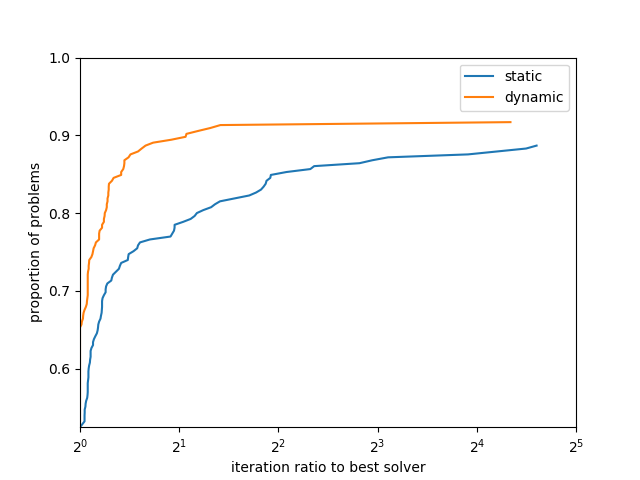
\includegraphics[scale=0.5]{ratios-dynamic-static.png}
%\caption{Comparison of dynamic and static $\mu$ updates for the one-phase algorithm.}
%\end{figure}

Figure~\ref{fig:alg-options} we trial different algorithm options. First, in the graph on the far left, we trial different line search conditions for the stabilization steps. In particular, we compare the default setting of a `filter' as described in line~\ref{line:filter} of Algorithm~\ref{alg:stable} against other possible conditions. The first baseline to replace this filter condition with  \eqref{eq:phi-sufficient-progress}, i.e., check that sufficient progress is made on the `log barrier' merit function. The other baseline is removing the filter condition entirely and simple taking the maximum step possible. Figure~\ref{fig:alg-options} indicates that the filter has superior performance of these three options. Note that Figure~\ref{fig:alg-options} (and other following figures) uses the performance profiling of \citet*{dolan2002benchmarking}. In particular, on the $x$-axis we plot:
$$
\frac{\text{iteration count of solver}}{\text{iteration count of fastest solver}}
$$
and the curve plotted is a cumulative distribution over the test set.

\begin{figure}[H]
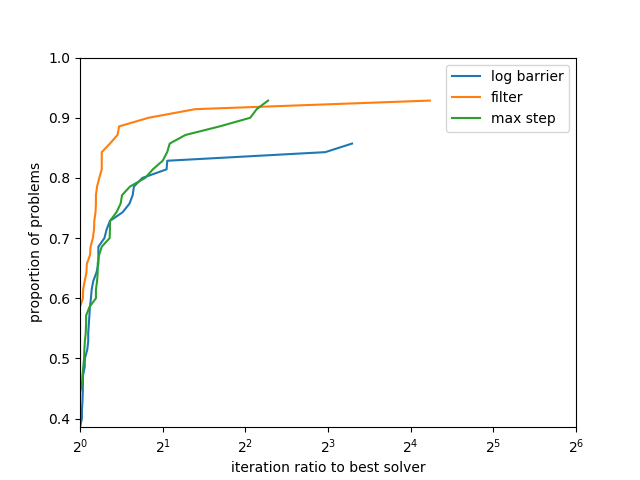
\includegraphics[scale=0.35]{ls-options.pdf}
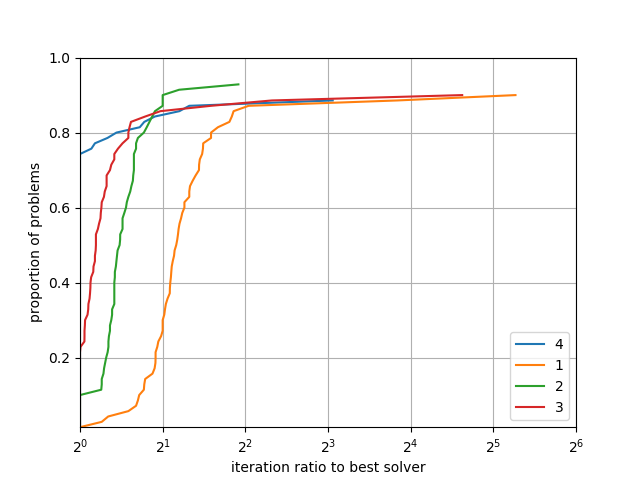
\includegraphics[scale=0.35]{num-corrections.pdf}
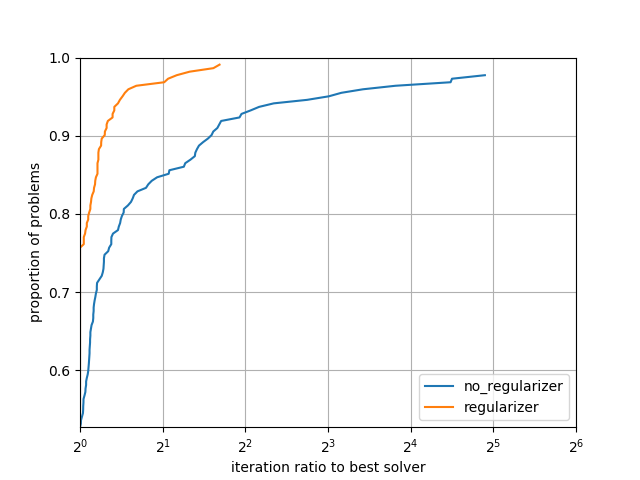
\includegraphics[scale=0.35]{regularizer-ratios.pdf}
\caption{Comparison of different algorithm options for the one-phase algorithm. Left, comparison of different line search options. Center, comparison of choice of for the parameter $\parNumCor$. Right, the algorithm with and without the regularizer.}
\label{fig:alg-options}
\end{figure}

In the graph in the center of Figure~\ref{fig:alg-options} we compare different choices of the parameter $\parNumCor$, the maximum number of corrections ($\parNumCor$ is used on line~\ref{take-steps} in Algorithm~\ref{one-phase-IPM}). As one would expect, increasing the number of corrections decreases the iteration count, but has little impact on the failure rate. In the actual implementation of our one-phase algorithm we chose $\parNumCor=\parNumCorValue$. Finally, the graph on the right shows that the regularizer helps improve performance.

\subsection{Comparison with IPOPT}\label{alg:comparison-IPOPT}

\hinder{compare only on problems where on solver finds an optimal solution}

For the comparisons we use IPOPT version 3.12.4 with the linear solver MUMPS \cite{amestoy1998mumps}. We turn off the nlp scaling, set the termination tolerance to $10^{-6}$ and set the boundary relaxation factor to zero. For both the one-phase algorithm and IPOPT we set the time limit to 1 hour and the maximum number of iterations $\parMaxItValue$. Currently, our code is written in Julia (using the default Cholesky factorization solver) and is not fully optimized for speed. Consequently, especially on small problems, it is slower than IPOPT. For some large-scale problems it is more competitive as we show in Section~\ref{sec:large-scale}. Therefore, for the CUTEst problems, we compare on the number of iterations rather than runtime. 

%Ideally, we would compare based on the number of factorizations because for large-scale problems this is, often, the most computationally intensive.


We consider the final function values $f_{A}^{*}$ and $f_{B}^{*}$ of algorithm $A$ and $B$ respectively approximately the same if:
$$
\frac{f_{A}^{*} - f_{B}^{*}}{1 + \max \{ | f_{A}^{*} |, | f_{B}^{*} | \} } < 10^{-1},
$$
otherwise, we consider the solution of algorithm $A$ better than algorithm $B$ if $f_{A}^{*}  < f_{B}^{*}$. For problems where both algorithms find a KKT point is reported in the top three rows of Table~\ref{tbl:pairwise-outcomes}. The remainder of Table~\ref{tbl:pairwise-outcomes} shows the number of times both algorithms succeed, fail, or just one algorithm fails. We consider the algorithm to have succeeded if it produces either a certificate of first order local optimality, infeasibility or unboundedness. 

Let us highlight a few interesting facts from Tables~\ref{tbl:pairwise-outcomes}-\ref{tbl:failure-reasons}. The one-phase algorithm seems to find better KKT points on $13$ problems versus $2$ for IPOPT (Table~\ref{tbl:pairwise-outcomes}). Furthermore, IPOPT fails on $39$ problems compared with $21$ problems for the one-phase algorithm (Table~\ref{tbl:termination-status-counts}). A large proportion of these failures occur before IPOPT has started (Table~\ref{tbl:failure-reasons}).

\begin{table}[H]
\caption{Pairwise comparison of outcomes for IPOPT and the one-phase algorithm}\label{tbl:pairwise-outcomes}
\begin{tabular}{ c c r }
  One Phase &  IPOPT &  \# \\
  \hline
same KKT & - & 158  \\
- & better KKT & 2 \\
better KKT & - &  13 \\
\hline
Succeed & Succeed & 185 \\
Fails & Fails & 7 \\
Succeed & Fails &  32 \\
Fails & Succeed & 14 \\
\end{tabular}
\end{table}

%Table~\ref{tbl:termination-status-counts} displays the 

\hinder{present as bar chart? and maybe reduce to two tables.}

\begin{table}[H]
\caption{Termination status counts}\label{tbl:termination-status-counts}
\begin{tabular}{ c c c r }
 &  One Phase &  IPOPT &  \\
  \hline
KKT &  201 & 191 \\
unbounded & 4 & 0  \\
primal infeasible & 12 &  8 \\
fail & 21 & 39 \\
\end{tabular}
\end{table}

\begin{table}[H]
\caption{Failure reasons}\label{tbl:failure-reasons}
\begin{tabular}{ c c c r }
 &  One Phase & IPOPT \\
  \hline
max time & 10 & 9  \\
max iter &  3 & 3 \\
error before starting & 4 & 19 \\
error during algorithm & 4 & 8 \\
\hline
total & 21 & 39
\end{tabular}
\end{table}

Figure~\ref{fig:comparison-IPOPT-on-CUTEst} compares the iterations that IPOPT and the one-phase algorithm take to succeed (produce a certificate of first order local optimality, infeasibility or unboundedness) on the CUTEst test set. Note that the iteration counts for the solvers are similar, except that the one-phase solver fails less frequently.


\begin{figure}[H]
\includegraphics[scale=0.5]{ratios-IPOPT-one-phase.pdf}
\includegraphics[scale=0.5]{iterations-IPOPT-one-phase.pdf}
%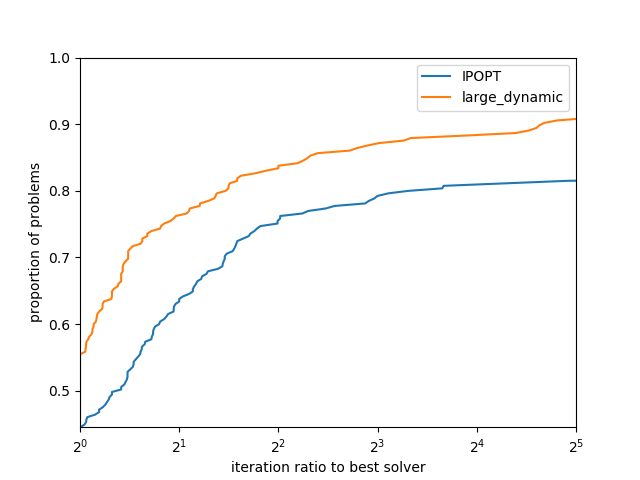
\includegraphics[scale=0.5]{ratios-n=50-10000.png}
%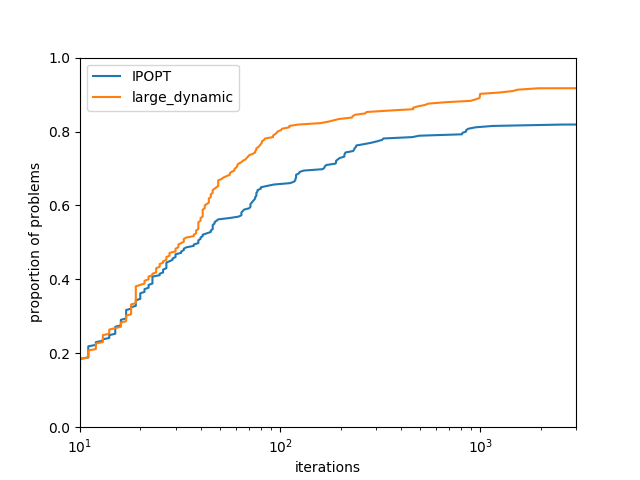
\includegraphics[scale=0.5]{iterations-n=50-10000.png}
\caption{Comparison of IPOPT and one-phase on CUTEst for problems where at least one solver declared the problem optimal, infeasible or unbounded.}\label{fig:comparison-IPOPT-on-CUTEst}
\end{figure}

\if\inProgress
\todo[inline]{table or plot of maximum dual variables? this would significantly strengthen case.}
\fi

\subsection{Comparison on infeasible problems}\label{sec:infeas}

Most of the CUTEst problems have feasible solutions. Recall that CUTEst writes problems in the form $l \le c(x) \le u$.
To generate a test set that was more likely to contain infeasible problems we shift the constraints as follows:
$$
\tilde{c}(x) = c(x) + e,
$$
and then input the problems to the one-phase solver and IPOPT. Note that the new problem may or may not be feasible.

The solver terminated with the statuses described in the Table~\ref{tbl:termination-status-counts-peturbed}. This test was only run on problems with at most $1,000$ variables and constraints total.
\begin{table}[H]
\caption{Termination status counts for perturbed CUTEst problems.}\label{tbl:termination-status-counts-peturbed}
\begin{tabular}{ c c c r }
 &  One Phase &  IPOPT &  \\
  \hline
KKT & 22 & 20 \\
unbounded & 1 & 0  \\
primal infeasible & 44 &  38 \\
fail & 3 & 12 \\
\end{tabular}
\end{table}

Next, in Figure~\ref{fig:comparison-IPOPT-on-perturbed-CUTEst} we compare IPOPT and the one-phase on the subset problems which at least one solver declared the problem locally infeasible. From this figure one can see that the one-phase solver is quicker and more robust than IPOPT.

\begin{figure}[H]
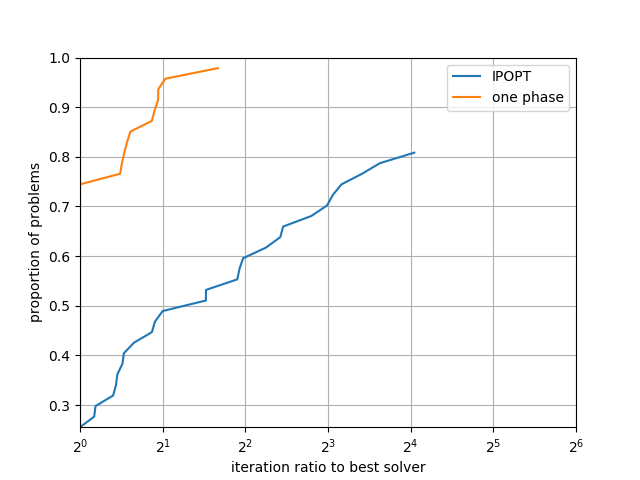
\includegraphics[scale=0.5]{infeas-ratios.png}
\caption{Comparison of IPOPT and one-phase on perturbed CUTEst problems for which at least one solver declares the problem locally infeasible.}\label{fig:comparison-IPOPT-on-perturbed-CUTEst}
\end{figure}

%
%\subsection{Comparison on NETLIB for linear programming}\label{sec:netlib}
%
%The purpose of this Section is to show that the one-phase algorithm has good performance on linear programs, as one would expect since the algorithm is heavily influenced by ideas from linear programming [REF]. My experience from our previous paper is that there is a huge difference in the performance of IPOPT and the one-phase algorithm.
%
%[Use IPOPT option specialized for LP]
%
%\begin{figure}[H]
%\missingfigure{...}
%%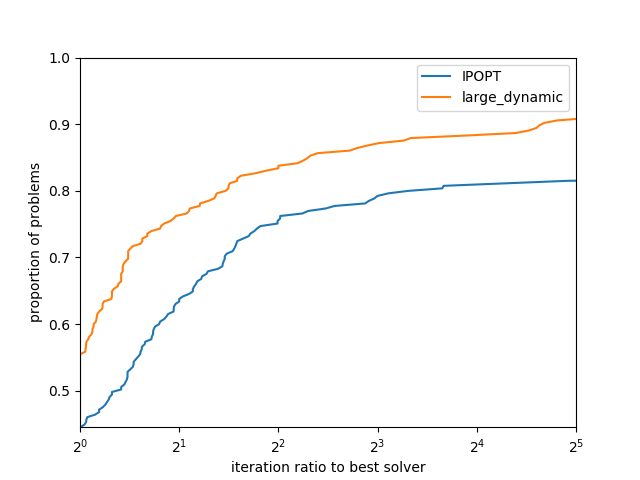
\includegraphics[scale=0.5]{ratios-n=50-10000.png}
%%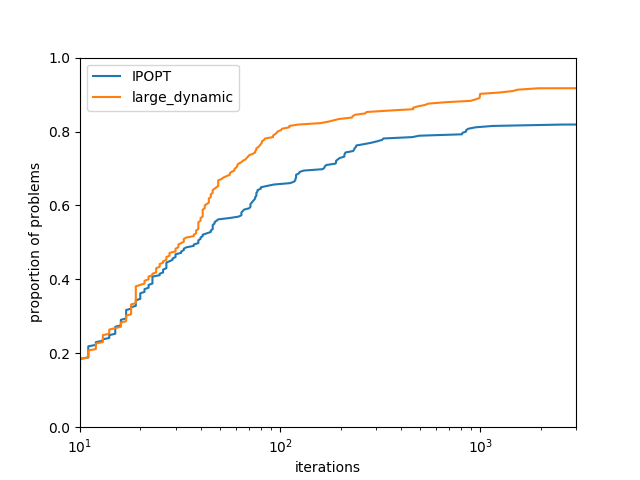
\includegraphics[scale=0.5]{iterations-n=50-10000.png}
%\caption{Comparison of IPOPT and one-phase on the NETLIB linear programming test set.}
%\end{figure}

\section{Comparison on selected large scale problems}\label{sec:large-scale}
\newcommand{\NETtimeOnePhase}{100}
\newcommand{\NETtimeIPOPT}{963}
\newcommand{\NETitOnePhase}{26}
\newcommand{\NETitIPOPT}{596}

Here we compare IPOPT and the one-phase solver on two large-scale problems. The goal is to highlight that, for certain large scale problems with amiable sparsity structure, the one-phase algorithm is vastly superior to IPOPT. The sizes of the problems are given in Table~\ref{large-scale:basic-info}. The first problem NET4 is the largest CUTEst problem (in terms of number of variables and constraints) with nonlinear constraints based on a real application. NET4 is a gas network problem for the British NTS system. Both IPOPT and the one-phase solve declare the problem infeasible, however, it takes the one-phase solver only 100 seconds ($26$ iterations) versus 963 seconds for IPOPT (596 iterations). This runtime difference can be put down to (i) the superior performance of the one-phase algorithm on infeasible problems and (ii) the constraints are sparse (see final column of Table~\ref{large-scale:basic-info}) which means $\Schur$ is very sparse, hence the factorizations of the one-phase algorithm is cheap. The second problem is a model of the economic impact of taxation decisions\footnote{Created by Micheal Saunders, Ding Ma and Kenneth Judd.}. This problem is (temporarily) generated with synthetic data. We have created three instances. A small, medium and large instance as recorded in Table~\ref{large-scale:basic-info} (ECON10, ECON50 and ECON250 respectively). Note that the problems have many more constraints than variables, this favors our approach of solving a linear system only the size of the number of variables instead of IPOPT's strategy of solving a system that is significantly larger. From Table~\ref{compare-runtime} one can see the one-phase solver has better runtime than IPOPT as the problem size increases.
\begin{table}[H]
\begin{tabular}{l l l l l l}
name &  \# vars & \# cons & \# nnz Hess & \# nnz Jac & \# nnz densest con  \\ 
NET4 & 61,488 & 75,024  & 151,056 & 247,557 & 12 \\  
ECON10 &  40 & 381 & 1,560 & 1,560 &  40 \\
ECON50 &  100 & 2,451 & 9,900 & 9,900 &  100 \\
ECON250 & 500 & 62,251 & 249,500 & 249,500 & 500 \\
\end{tabular}
\caption{Basic information on selected large-scale test problems}\label{large-scale:basic-info}
\end{table}


\begin{table}[H]
\begin{tabular}{|c| c c | c c |}
  \hline
  \multirow{2}{*}{} 
      & \multicolumn{2}{c|}{Time (s)} 
          & \multicolumn{2}{|c|}{\# iterations} \\             \cline{2-5}
  & one-phase & IPOPT & one-phase & IPOPT \\  \hline
  NET4 & $\NETtimeOnePhase$ & $\NETtimeIPOPT$  & $\NETitOnePhase$   & $\NETitIPOPT$ \\      \hline
    ECON20 & $2$  & $0$  & $73$ & $25$   \\      \hline
  ECON50 & $6$  & $335$  & $85$ & $122$   \\      \hline
  ECON250 & $412$  &  out of memory & $207$ & out of memory \\      \hline
\end{tabular}
\caption{Runtime comparison on selected large-scale test problems}\label{compare-runtime}
\end{table}


\if\inProgress1

\hinder{convert first two COPs problem into julia}

\section{Conclusions}
\begin{enumerate}
\item ??
\end{enumerate}


\section{To do}

\begin{enumerate}
\item clean up 
\item edit code to match document
\item run full CUTEst test
\item explain performance on Watcher-Beliger example.
\end{enumerate}

\fi

\hinder{Given a strictly feasible starting point, by setting $\conWeight = 0$ one can remain strictly feasible for the remainder of the algorithm. Maybe give an example problem.}

\hinder{If we set $\mu$ large and $\conWeight$ small then the algorithm is essentially a two-phase algorithm -- makes a lot of sense for problems with large interior. But works terribly for problems with a small interior.}

\section*{Acknowledgements}

We would like to thank Michael Saunders and Ron Estrin for useful conversations and feedback on the paper.

\bibliographystyle{abbrvnat} %abbrv}
\bibliography{library-one-phase-2.bib}


\appendix

%\section{Examples showing the importance of the regularizer}\label{app:examples-regularizer}
%
%This section gives examples showing that the regularizer is necessary to guarantee that each barrier sub-problem has a bounded optimal solution. Example~\ref{example-regular-1} shows that either $\parConRegularizer > 0$ or $\parRegularizer > 0$ is necessary, even for solving linear programs. Example~\ref{example-regular-2} shows that $\parRegularizer > 0$ is needed to ensure that the optimal solution of all sub-problems is bounded. Example~\ref{example-regular-3} shows that $\parConRegularizer > 0$ is needed to ensure that the optimal solution of all sub-problems is bounded.
%
%\begin{example}\label{example-regular-1}
%Consider the problem 
%$$\min{ 0 } \text{ s.t. }  x \le 0.$$ 
%For this problem with $\conWeight = [1]$ and $\parRegularizer = 0$, 
%$$\barrier_{\mu}(x) = \parConRegularizer \mu x - \mu \log(\mu - x)$$ 
%and the optimal solution is $x^{*} = \frac{1 + \parConRegularizer}{\parConRegularizer}$ for all $\mu$, alternately if $\parConRegularizer = 0$ then $x^{*} \rightarrow \infty$.
%\end{example}
%
%\begin{example}\label{example-regular-2}
%Consider the problem 
%$$\min{ \exp(x_{2}) } \text{ s.t. }  \exp(x_{1}) \le x_{2} - 1, x_{2} \ge 1.$$ 
%For this problem with $\conWeight = [1;~1]$, 
%$$\barrier_{\mu}(x) = \exp(x_{2}) + \mu r(x)  - \mu \log(\mu + x_{2}) - \mu \log \left(\mu + x_{2} - 1 - e^{x_{1}}\right).$$ 
%If $\parRegularizer = 0$, $\parConRegularizer > 0$ then for sufficiently large $\mu$ the optimal solution is $x_{1} \rightarrow \infty$, $x_{2} = 0$.
%\end{example}
%
%\begin{example}\label{example-regular-3}
%Consider the problem
%$$
%\min{x/2} \text{ s.t. } 1 - \exp(x^2) \le 0.
%$$
%For this problem with $\conWeight = [1]$,
%$$\barrier_{\mu}(x) = x/2 + \mu r(x)  - \mu \log(\mu + \exp(x^2) - 1) .$$ 
%If $\mu = 1$, $\parConRegularizer = 0$ and $\parRegularizer > 0$ then
%$$\barrier_{1}(x) = x/2 + \sqrt{\parRegularizer x^2 + 1}  - x^2$$ 
%which is unbounded below.
%\end{example}

\section{Global convergence proofs for Algorithm~\ref{simple-one-phase}}\label{app:global-conv}

The purpose of this section is to provide proofs for supporting results for Theorem~\ref{thm:global-convergence}.

\subsection{Convergence of aggressive steps}


\subsubsection{Proof of Lemma~\ref{lemma:agg-succeeds}}\label{sec:lemma:agg-succeeds}

\lemAggSucceeds*
\begin{proof}
First, observe that as $\delta \rightarrow \infty$ the direction $\dir{x}$ computed from \eqref{eq:Schur-complement-system} tends to zero. Consider any $\alpha_{P} \in (0,1)$, since the function $a$ is continuous for sufficiently large $\delta$ we have
\begin{flalign}\label{eq:a-bound}
\| \cons(x) - \cons(x + \alpha_{P} \dir{x}) \|_{\infty} \le \frac{\parCompAgg - \parComp}{2 \parCompAgg} \min_i\{ s_{i} \}.
\end{flalign}

%To obtain a contradiction assume that Algorithm~\ref{alg:simple-agg-step} fails. This implies that for
Consider what occurs when we set
\begin{flalign}\label{eq:alpha-bound}
\alpha_{P} = \minStepFunc(\mu, s) = \min_{i : w_i > 0}{ \frac{(\parCompAgg - \parComp) s_{i}}{2  \parCompAgg \mu \conWeight_i} } 
\end{flalign}
then for this choice of $\alpha_{P}$ we have
$$
\| s^{+} - s \|_{\infty} = \|  -\alpha_{P} \mu\conWeight+  \cons(x) - \cons(x + \alpha_{P} \dir{x}) \|_{\infty} \le  \alpha_{P} \mu \|  \conWeight \|_{\infty} +  \| \cons(x) - \cons(x + \alpha_{P} \dir{x}) \|_{\infty} \le \frac{\parCompAgg - \parComp}{\parCompAgg} \min_i\{ s_{i} \},
$$
where the first equality holds by \eqref{eq:slackVarUpdate} and final inequality holds by \eqref{eq:a-bound} and \eqref{eq:alpha-bound}.
Note that 
$$
\frac{s^{+} Y}{\mu} = \frac{S Y}{\mu} (e + S^{-1} (s^{+} - s)) \in \left[  \frac{\parComp}{\parCompAgg}, \frac{\parComp}{\parCompAgg} \right] \frac{s Y}{\mu} \subseteq e  [\parComp, 1/\parComp ].
$$
where the second transition follows from substituting our bound on $\| s^{+} - s \|_{\infty}$ and for the upper bound using $\frac{\parCompAgg - \parComp}{\parCompAgg} < \frac{\parCompAgg - \parComp}{\parComp}$, the final transition uses $ \frac{s Y}{\mu} \in e [\parCompAgg, 1/\parCompAgg]$.

Therefore $\alpha_{D} = 0$ gives a feasible dual iterate. We conclude there exists a $\delta$ such that the $\alpha_{P}$ chosen by line~\ref{simple-agg-select-alpha-P} is at least $\minStepFunc(\mu, s)$, which proves the result.
\end{proof}


\subsubsection{Proof of Lemma~\ref{lem:yw-bounded}}\label{sub:lem:yw-bounded}

\lemYWbounded*

\begin{proof}
Since \eqref{terminate-primal-infeasible} does not hold: either $a(x)^T y \le 0$,
$\infeasFuncOne (\mu,x,s,y) > \TOLinfOne$ or $\infeasFuncTwo (\mu,x,s,y) > \TOLinfTwo$. We consider these possibilities in order.

If $a(x)^T y \le 0$ then $(\mu \conWeight - s)^T y = a(x)^T y \le 0$ by $\cons(\vec{x}) + \vec{s} = \mu \conWeight$ which implies $y^T \conWeight \le s^T y / \mu \le m / \parComp$.

If $\TOLinfOne < \infeasFuncOne (\mu,x,s,y) = \frac{\| \grad  a(x)^T y \|_{1}}{ a(x)^T y }$ then
\begin{flalign*}
w^T y &< s^T y + \frac{\| \grad  a(x)^T y \|_{1}}{ \TOLinfOne  } \le s^T y + \frac{\| \grad f(x) + \parComp \mu e^T \grad a(x) \|_{1} + \| \grad \Lag_{\mu}(x,y) \|_{1}}{ \TOLinfOne  } \\
&\le s^T y + 2 \frac{\| \grad f(x) + \parComp \mu e^T \grad a(x) \|_{1}}{ \TOLinfOne  } 
\end{flalign*}
where the first inequality holds by re-arranging, the second by the triangle inequality and the third by the assumption that the aggressive step criteron \eqref{agg-criteron-farkas} is met. Furthermore, the term $s^T y$ is bounded by $\mu / \parCompAgg$ and the term $\| \grad f(x) + \parComp \mu e^T \grad a(x) \|_{1}$ is bounded because $f$ and $a$ are twice differentiable and the unboundness criterion~\eqref{terminate-dual-infeasible} is not met.

\item Neither the infeasibility termination criterion~\eqref{terminate-primal-infeasible} or the unboundness criterion~\eqref{terminate-dual-infeasible} are met.

If $\TOLinfTwo < \infeasFuncTwo (x,s,y)  = \frac{\| \grad  a(x)^T y \|_{1} + s^T y}{ \| y \|_{1} }$ then
\begin{flalign*}
\| y \|_{1} &<  \frac{s^T y + \| \grad  a(x)^T y \|_{1}}{\TOLinfTwo} \le \frac{ s^T y + \| \grad f(x) + \parComp \mu e^T \grad a(x) \|_{1} + \| \grad \Lag_{\mu}(x,y) \|_{1}}{\TOLinfTwo} \\
&\le 2 \frac{ s^T y + \| \grad f(x) + \parComp \mu e^T \grad a(x) \|_{1}}{\TOLinfTwo}
\end{flalign*}

where the first inequality holds by re-arranging, the second by the triangle inequality and the third by the assumption that the aggressive step criteron \eqref{agg-criteron-farkas} is met.
We conclude $\| y \|_{1}$ is bounded since $\| x \|$ is bounded, clearly therefore $w^T y$ is also bounded above.

Since in all three cases $\conWeight^T y$ is bounded we conclude the proof.
\end{proof}


\subsection{Convergence results for stabilization steps}

\subsubsection{Proof of Lemma~\ref{lem:compact-Q} and Corollary~\ref{coro:bound-everything}} \label{sec:lem:compact-Q}


We now introduce the set $\mathbb{Q}_{\mu, C}$ which we will use to represent the set of possible points the iterates of Algorithm~\ref{simple-one-phase} can take for a fixed $\mu$, i.e., during consecutive stabilization steps.

\begin{definition}\label{defQ}
Define the set $\mathbb{Q}_{\mu, C}$ for constants $\mu, C > 0$ as the set of points $(x,y,s) \in  \R^{\nvar} \times \R^{\ncon++} \times \R^{\ncon++}$ such that assumption~\ref{assume:primal-feasible} holds and
\begin{enumerate}
\item \label{Q-phi-bounded-above} The function $\phi_{\mu}$ is bounded above, i.e., $\phi_{\mu}(x,y,s) \le C$.
\item \label{Q-bounded-below} The primal iterates are bounded, i.e., $\| x \| \le C$. 
\end{enumerate}
\end{definition}

Suppose Algorithm~\ref{simple-one-phase} generates consecutive stabilization steps stabilization steps $(\mu^k, x^k, s^k, y^k)$ for $k \in \{ \kStart, \dots, \kEnd \}$ with $\mu =\mu^{\kStart} = \dots = \mu^{\kEnd}$ and none of these iterates satisfy the unboundedness termination criterion~\eqref{terminate-dual-infeasible}. Let us show these iterates are contained in $\mathbb{Q}_{\mu, C}$, i.e., $(x^{k}, s^{k}, y^{k}) \in \mathbb{Q}_{\mu, C}$ for some $C > 0$. For $C \ge  \phi_{\mu}(x^{\kStart}, s^{\kStart}, y^{\kStart})$ condition \ref{defQ}.\ref{Q-phi-bounded-above} holds since during stabilization steps we only accept steps that decrease $\phi_{\mu}$. For sufficiently large $C$, condition \ref{defQ}.\ref{Q-bounded-below} holds from the assumption the unboundedness termination criterion~\eqref{terminate-dual-infeasible} is not satisfied.



We are now ready to prove Lemma~\ref{lem:compact-Q}. Note that during Lemma~\ref{lem:compact-Q} we will repeatedly use that the following elementary real analysis fact: 

\begin{fact}
Let $X = \{ x : g_i(x) \le 0 \}$. If $g_i$ is a continuous function and the set $X$ is bounded, then the set $X$ is compact.
\end{fact}

\begin{restatable}{lemma}{lemCompactQ}\label{lem:compact-Q}
Suppose assumptions~\ref{assume:diff} and \ref{assume:parameters} hold. 
For any constants $C, \mu > 0$ the set $\mathbb{Q}_{\mu, C}$ is compact.
\end{restatable}

\begin{proof}
First consider the set
$$
Q := \left\{ x \in \R^{\nvar} : (y, s) \in \R^{\ncon++} \times \R^{\ncon++}, \phi_{\mu}(x,y,s) \le C, \| x \| \le C \right\} 
$$
By $\| x \| \le C$ we see $Q$ is bounded. Furthermore, since $\phi_{\mu}(x) \le C$ and $Q$ is bounded there exists some constant $K_{1} > 0$ such that
$$
\mu w - \cons(x) \ge K_{1}
$$
for all $x \in Q$. Consider some sequence $x^{k} \in Q$ with $x^{k} \rightarrow x^{*}$. The statement $\cons(x) \le \mu w - K_{1}$ implies $\phi_{\mu}$ is continuous in a neighborhood of $x^{*}$. Using the definition of $Q$ and the assumption that $f$ and $a$ are continuous implies $x^{*} \in Q$, i.e., $Q$ is compact. 


%Using the fact that $Q$ is compact and $s > 0$ we deduce that $S^{-1} e$ is bounded, it follows that
Note that:
$$
\mathbb{Q}_{\mu, C} = \left\{ (x,y,s) \in \R^{\nvar} \times \R^{\ncon++} \times \R^{\ncon++} : x \in Q, \cons(x) + s = \mu \conWeight, \frac{S y}{\mu} \in [\parComp e, \ones / \parComp]\right\}.
$$
Consider some $(x,y,s) \in \mathbb{Q}_{\mu, C}$, since $s = \mu w - \cons(x) \ge K_{2}$ and $\frac{S y}{\mu} \in [\parComp e, \ones / \parComp]$ we can deduce $y$ is bounded. Since the function $\cons(x)$ and $S y$ are continuous we conclude $\mathbb{Q}_{\mu, C}$ is compact.
\end{proof}

\begin{restatable}{corollary}{coroBoundEverything}\label{coro:bound-everything}
Assume the functions $f : \R^{\nvar} \rightarrow \R$ and $a : \R^{\nvar} \rightarrow \R^{\ncon}$ be twice differentiable on $\R^{\nvar}$. Consider some fixed $\mu \in (0, \mu^0]$ and $C \in \R$.
Then there exists some $L > 0$ such that for all $(x, s, y) \in \mathbb{Q}_{\mu, C}$ the following inequalities hold:
$$
s_i, y_i \ge 1/L
$$
$$
\| x \|, \| y \|, \| s \|, \| \grad \barrier_{\mu}(x) \|, \| \Schur \|, \| \grad \cons(x) \| \le L
$$
and for any $d$ s.t. $\| u \| < 1 / L$
\begin{subequations}\label{lipschitz-continuous}
\begin{flalign}
\barrier_{\mu}(x + d) &\le \barrier_{\mu}(x) + \grad \barrier_{\mu}(x)^T d + L / 2 \| d \|^2 \label{phi-lipschitz-continuous} \\
\| \cons(x) + \grad \cons(x) u -\cons(x + u)  \| &\le L  \| u \|^2. \label{a-lipschitz-continuous-2nd}
\end{flalign}
\end{subequations}

Furthermore, if the aggressive criterion~\eqref{agg-criteron} does not holds then
$$
\max\{ \| \grad \barrier_{\mu}(x) \|, \| S y - \mu \|_{\infty} \} \ge 1 / L.
$$
\end{restatable}

\begin{proof}
All these claims use Lemma~\ref{lem:compact-Q} and the elementary real analysis fact that for any continuous function $g$ on a compact set there $X$ there exists some $x^{*} \in X$ such that $g(x^{*}) = \sup_{x \in X}{g(x)}$.

The only non-trivial claim is showing \eqref{lipschitz-continuous}, which proceed to show. Since there exists some constants $\varepsilon_{1} > 0$ such that $(x,y,s) \in \mathbb{Q}_{\mu, C}$ we have $\cons(x) \le \mu w - \varepsilon_{1}$. It follows that there exists some constant $\varepsilon_2 > 0$ such that for all $\| u \| \le \varepsilon_2$ we have $\cons(x + u) < \mu w$. It follows that there exists some $L > 0$ such that $\| \grad^2 \barrier_{\mu}(x) \| \le L$.

For some $x$ and $\nu$ with $\| \nu \| = 1$ define the one dimensional function
$$
h(\alpha) :=  \barrier_{\mu}(x + \alpha \nu) 
$$
then for $\alpha \in [0, \varepsilon_2]$ we get
$$
h(\alpha) - h(0) - \alpha h'(0) = \int_{0}^{\alpha}{ \int_{0}^{\eta_{2}}{h''(\eta) \partial \eta_{1} \partial \eta_{2}} } \le \alpha^2 L / 2,
$$
which using $u = \nu \alpha$ for $\alpha \in [0, \varepsilon_2]$ concludes the proof of \eqref{phi-lipschitz-continuous}. Showing \eqref{a-lipschitz-continuous-2nd} consists of a similar argument.
\end{proof}

%With Corollary~\ref{coro:bound-everything} in hand we proceed to showing for sufficiently large $\delta$, Algorithm~\ref{alg:stable} will succeed.
%that there will only be a finite number of stabilization steps until the next aggressive step.


\subsubsection{Proof of Lemma~\ref{lemConsecutiveStable}}\label{sec:lemConsecutiveStable}

We remark that Lemma~\ref{lemConsecutiveStable} uses Lemma~\ref{lem:compact-Q} and Corollary~\ref{coro:bound-everything} which are proved in Section~\ref{sec:lem:compact-Q}

\lemConsecutiveStable*

\begin{proof}
Recall that, as we discussed following Definition~\ref{defQ}, there exists some $C > 0$ such that for any consecutive series of stabilization steps $(\mu^k, x^k, s^k, y^k)$ for $k \in \{ \kStart, \dots, \kEnd \}$ we have $(x^k, s^k, y^k) \in \mathbb{Q}_{\mu, C}$ with $\mu = \mu_{k_{\kStart}} = \mu_{k_{\kEnd}}$.


From Corollary~\ref{coro:bound-everything} we know that $\lambda_{\max}(\Schur) \le L$, therefore 
\begin{flalign*}
\dir{x}^T \grad \psi(x) = -\grad \psi(x)^T (\Schur + \delta I)^{-1} \grad \psi(x) \le -\| \grad \psi(x) \|^2 / (L + \delta) \le -\| \grad \psi(x) \|^2 / (3 L + \mu),
\end{flalign*}
where the first transition uses the definition of $\dir{x}$ in \eqref{eq:Schur-complement-system} with $\gamma = 1$ when computing $b$, the second transition $\lambda_{\max}(\Schur) \le L$ and the third transition uses $\delta \le 2 L + \mu$ from line~\ref{alg-simple-delta-min} of Algorithm~\ref{simple-one-phase}.

Similarly, by line~\ref{alg-simple-delta-min} of Algorithm~\ref{simple-one-phase} we get
\begin{flalign*}
\| \dir{x} \|^2 = \| (\Schur + \delta I)^{-1} \grad \psi(x)\|^2 \le \| \grad \psi(x)\|^2 / \mu.
\end{flalign*}

Furthermore,
\begin{flalign*}
\barrier_{\mu}(x^{+}) - \barrier_{\mu}(x)  &\le \alpha_{P} \grad \barrier_{\mu}(x)^T \dir{x} + L \alpha_{P}^2 \| \dir{x} \|^2 \\
&\le \alpha_{P} \left( \parObjReductFactor \grad \barrier_{\mu}(x)^T \dir{x} + \| \grad \barrier_{\mu}(x)\|^2 \left(  \frac{\alpha_{P} L}{\mu} - \frac{1}{4L + 2 \mu} \right)  \right) \\
&= \alpha_{P} \left( \parObjReductFactor \grad \barrier_{\mu}(x)^T \dir{x} + \| \grad \barrier_{\mu}(x)\|^2 \left(  \frac{\alpha_{P} (L +  \delta / 2)}{\mu} - \frac{1}{8L + 4\mu} \right) - \| \grad \barrier_{\mu}(x)\|^2 \frac{1}{8L + 4\mu} - \frac{\alpha_{P} \delta}{2} \| \dir{x} \|^2 \right) \\
&\le \parObjReductFactor \alpha_{P} \left( \grad \barrier_{\mu}(x)^T \dir{x} - \frac{\alpha_{P}  \delta}{2} \| \dir{x} \|^2 - c_{1} \| \grad \barrier_{\mu}(x)\|^2  \right) 
\end{flalign*}
where the first inequality holds by Corollary~\ref{coro:bound-everything}, the second by the above inequalities, the third by adding and subtracting terms, the fourth for sufficiently small $\alpha_{P} > c_{1}$ and constant $c_{1} > 0$.

We can bound $\| \dir{x} \|$, $\| \dir{y} \|$ and $\| \dir{s} \|$ using our bound on $\| \dir{x} \|$, Corollary~\ref{coro:bound-everything} and \eqref{compute-ds-dy}.

Finally,
\begin{flalign*}
\| S^{+} y^{+} - \mu \|_{\infty}  &\le \| S y - \mu \|_{\infty} + \alpha_{P} \left( -\| S y - \mu \|_{\infty} + \alpha_{P} L \| \dir{x} \|^2 \| y^{+} \|_{\infty} + \alpha_{P} \| \dir{s} \|_{\infty} \| \dir{y} \|_{\infty} \right) \\
&\le  \| S y - \mu \|_{\infty} (1 - \alpha_{P}  + c_{2} \alpha_{P}^2 )
\end{flalign*}
where the first inequality holds by $S y + S \dir{y} + Y \dir{s} = \mu$ and Corollary~\ref{coro:bound-everything}, \eqref{a-lipschitz-continuous-2nd}, which shows $\| s + \dir{s} - s^{+}  \|_{\infty} \le L \| \dir{x} \|^2$, the second by the fact that the directions and $\| y \|$ are bounded.

Using $\MeritComp_{\mu}(s,y) = \frac{\| S y - \mu \|_{\infty}^3}{\mu^2}$ we get
$$
\MeritComp_{\mu}(s^{+},y^{+}) \le \MeritComp_{\mu}(s,y) (1 - \alpha_{P}) + \bar{c}_{2} \alpha_{P}^2.
$$
Defining
$$
\Upsilon(\alpha_{P}) := \alpha_{P} \parObjReductFactor \left( \frac{1}{2} \left( \grad \psi_{\mu}(x)^T  \dir{x} - \frac{\delta}{2} \alpha_{P} \norm{ \dir{x}}^2 \right) -  \MeritComp_{\mu}(s,y)  \right),
$$
we get
\begin{flalign*}
\phi_{\mu}(x^{+},y^{+},s^{+}) - \phi_{\mu}(x,y,s) &\le \Upsilon(\alpha_{P}) + \alpha_{P} \left( c_{2} \alpha_{P}  - c_{3} \MeritComp_{\mu}(s,y) - c_{1} \| \grad \barrier_{\mu}(x)\|^2 \right).
\end{flalign*}
Since $\max\{ \MeritComp_{\mu}(s,y), \| \grad \barrier_{\mu}(x)\| \}$ is bounded away from zero, we deduce the largest $\alpha_{P}$ satisfying $\phi_{\mu}(x^{+},y^{+},s^{+}) - \phi_{\mu}(x,y,s) \le \Upsilon(\alpha_{P})$ is bounded away from zero. We conclude that we must reduce $\phi_{\mu}$ by a constant amount each iteration, which means that if there is an infinite sequence of stabilization steps then $\phi_{\mu}(x^k, s^k, y^k) \rightarrow \infty$ and hence $\| x^k \| \rightarrow \infty$.
\end{proof}

\if\inProgress1

\section{Super-linear convergence}\label{app:superlinear-conv}


\hinder{currently re-writing these results}

\hinder{
one can get super-linear convergence purely through the aggressive steps, just take a step size $\alpha = 1 - \mu^{\theta}$ with $\theta \in (0,1)$. 
eat into boundary.
}
\hinder{add switching condition for super-linear mode i.e. $\mu^{+} \le \mu^{\theta}$ and $\| \grad \Lag_{\mu}(x^{+},y^{+}) \| \le \mu^{\theta}$.}

\hinder{look at old paper}

\subsection{Proof of Lemma~\ref{lemDirectionSize}}\label{sec:lemDirectionSize}

Consider the following two Lemmas. 

\begin{lemma}\label{lem:hager-reformulated}
Suppose Assumption~\ref{second-order-sufficient-conditions} holds then there exists a neighborhood $N$ of $(x^{*},s^{*},y^{*})$ such that for all $(x,s,y) \in N$  if $ \| \grad_{x} \Lag_{\mu}(x,y) \|  = O(\mu)$ there exists $\tilde{y}^{*}$ with such that $\grad \Lag(x^{*}, \tilde{y}^{*}) = 0$ and 
$$\| (x,s,y) - (x^{*}, s^{*}, \tilde{y}^{*}) \|  = O( \mu ).$$
\end{lemma}

\begin{proof}
Follows from \citet{hager1999stability}.
\end{proof}


\begin{restatable}{lemma}{lemDistanceToDirection}\label{lemDistanceToDirection}
Assume $M > 0$ at $x$ etc. Then for any KKT point $(x^{*}, s^{*}, y^{*})$ and $(x,s,y)$ with $\norm{ (x^{*}, s^{*}, y^{*}) - (x,s,y)} = O(\mu)$ directions $\dir{}$ computed via \eqref{eq:Schur-complement-system} and \eqref{compute-ds-dy} with  $\gamma = 0$ satisfy 
$$\| \dir{} \| = O \left( \mu \right).$$
\end{restatable}


We defer the proof of Lemma~\ref{lemDistanceToDirection} to Section~\ref{sec:lemDistanceToDirection}.
Combining these two Lemma allows us to deduce Lemma~\ref{lemDirectionSize}.

\lemDirectionSize*

\begin{proof}

\end{proof}


\subsection{Proof of Lemma~\ref{lemDistanceToDirection}}\label{sec:lemDistanceToDirection}

\begin{lemma}\label{matrix-bound-lemma}
Consider matrices $H  \in \R^{\nvar \times \nvar}$, $A \in \R^{\nvar \times \ncon}$ and $D \in \R^{\ncon \times \ncon}$ with $H$ and $D$ symmetric, and vector $v \in \R^{\nvar}$. Let $M = H + A^T D^2 A$. Consider a vector $u^{*} \in \R^{\ncon}$ that solves
$$
M u^{*} =  v
$$
then 
%$$\| u^{*} \|^2 \le \frac{16 \| r \|^2}{ \lambda_{\min}(M)}  \max\left\{1, \frac{- \lambda_{\min}(H)}{\lambda_{\min}(M)} \right\}.$$
$$\| D A u^{*} \| \le 8 \| v \| \max\left\{1, \frac{- \lambda_{\min}(H)}{\lambda_{\min}(M)} \right\}.$$
\end{lemma}

\begin{proof}
\hinder{is there a simpler argument?}
Note that since $\lambda_{\min}(M) \ge 0$ we deduce $u^{*}$ is the minimizer of $g(u) := u^T M u +  2 u^T A^T D r$, furthermore for any $\eta \in \R$ we have
$$
g(u)  = (1 - \eta) u^T M u + \eta u^T H u + \eta \| D A u -  v / \eta \|^2 - \| v \|^2 / \eta.
$$
If $\eta = 1/4 \min\left\{1,  \frac{-  \lambda_{\min}(M)}{\lambda_{\min}(H)} \right\}$ then
$$
0 = g(0) \ge g(u^{*}) \ge \| u^{*} \|^2 ( \lambda_{\min}(M) / 2 + \eta \lambda_{\min}(H) ) + \eta \| D A u^{*}  -  v / \eta \|^2 - \| v \|^2 / \eta \ge   \eta \| D A u^{*}  -  v / \eta \|^2  - \| v \|^2 / \eta 
$$
%and $\| D A u -  r / \eta \| \ge 0$
where the second inequality holds using $\eta \le 1/2$, the final inequality uses $\eta \le -\lambda_{\min}(M) / (4 \lambda_{\min}(H))$. Re-arranging this equation and applying the triangle inequality gives
$$
\| D A u^{*} \|^2 \le 2 \| v \|^2 / \eta^2
$$
substituting for $\eta$ gives the result.
\end{proof}

\begin{lemma}\label{generic-direction-bound}
\hinder{under generic neighborhood assumption}
Assume $\lambda_{\min}(\Schur) > c_{1} > 0$, $\lambda_{\min}( \grad^2 \Lag_{\mu}(x,y) ) > c_{2}$, $\| y \| < c_{3}$ and $\mu \in (0,1)$. If $\hat{d}$ satisfies
$$\mathcal{K}_{0} \hat{d} = b$$
then
$$
\| \hat{d} \| = O \left( \frac{\| b \|}{\mu} \right).
$$
\end{lemma}

\begin{proof}
Recall from \eqref{eq:Schur-complement-system} that with $\delta = 0$ the direction $\dir{x}$ satisfies:
$$
\Schur \dir{x} = -\left( b_{D} + \grad \cons(x)^T S^{-1} \left( Y b_{P} - b_{C} \right) \right).
$$
since $\| b_{D} + \grad \cons(x)^T S^{-1} \left( Y b_{P} - b_{C} \right) \| = O( \| b \| / \mu)$ we get
$$
\| \dir{x} \| = O( \| b \| / \mu).
$$

Furthermore, by \eqref{compute-ds-dy} we have
$$
\| \dir{s} \| \le \| b_{P} \| + \| \grad \cons(x) \dir{x} \| = O( \| b \| / \mu )
$$
$$
\| \dir{y} \| = \| S^{-1/2} Y^{1/2} \| \| S^{-1/2} Y^{1/2} \grad \cons(x) \dir{x} \| + O(  \| b \| / \mu) = O(  \| b \| / \mu)
$$
where the last transition follows by Lemma~\ref{matrix-bound-lemma}.
\end{proof}



\lemDistanceToDirection*

\begin{proof}
Let $\tilde{d} = (x,s,y) - (x^{*}, s^{*}, y^{*})$ and $\hat{b} = \mathcal{K}_{0} \tilde{d} - b$. Note that
$$
\| \mathcal{K}_{0} \tilde{d} - b \| = \| \hat{b} \| = O( \| \tilde{d} \|^2 )
$$
Let $\hat{d}$ be a solution to $\mathcal{K}_{0} \hat{d} = \hat{b}$ by Lemma~\ref{generic-direction-bound} we have
$$
\| \hat{d} \| = O ( \| \hat{b} \| / \mu ) = O( \| \tilde{d} \|^2 / \mu ) = O(\mu)
$$
\end{proof}


\subsection{Proof of Theorem~\ref{thmSuperlinear}}\label{sec:thmSuperlinear}
\begin{lemma}
Let $\tau = \frac{\parComp + \parCompAgg}{2}$.
Suppose Assumption~\ref{second-order-sufficient-conditions} holds at the point $(x^{*}, s^{*}, y^{*})$. Then there there exists some radius $R > 0$, such that then for all $r \in (0,R)$  if the iterates begin with $\norm{ (0,x^{*},s^{*},y^{*}) - (\mu,x,s,y) } < r$ and $Sy / \mu \in [\parCompAgg, 1/\parCompAgg]$ then the consecutive sequence of aggressive steps starting at $(\mu,x,s,y)$ we have
\begin{enumerate}
\item $\norm{ (0,x^{*},s^{*},y^{*}) - (\mu, x,s,y) } < 2 r$
\item $Sy / \mu \in [\tau, 1/\tau]$
\end{enumerate}
\end{lemma}

\begin{proof}

\end{proof}

\thmSuperlinear*

\begin{proof}

\end{proof}

\fi

\section{Matrix factorization strategy}

\hinder{re-write and add initialization scheme}


This strategy is based on the ideas of IPOPT \cite[Algorithm IC]{wachter2006implementation}.

\begin{algorithm}[H]
\textbf{Input:} The matrix $\Schur$ and current delta choice $\delta$ \\
\textbf{Output:} The factorization of $\Schur +  \delta \eye$ for some $\delta > 0$ such that the matrix $\Schur +  \delta \eye$ is positive definite.
\begin{enumerate}[label*=A.{\arabic*}]
\item Set $\deltaPrev \gets \delta$
\item Set $\delta \gets 0$
\item Perform Cholesky factorization of $\Schur$, if inertia is correct return factorization $\Schur$ otherwise continue.
\item If $\deltaPrev > 0$ set $\delta \gets \max\{ \parDeltaMin, \deltaPrev \parDeltaDecrease \}$ otherwise set $\delta =\parDeltaStart$.
\item Perform Cholesky factorization of $\Schur + \delta \eye$, if inertia is correct return factorization of $\Schur + \delta \eye$ otherwise continue.
\item Set $\delta \gets \parDeltaIncreaseFailure \delta$. Go to previous step.
\end{enumerate}
\caption{Matrix factorization strategy}\label{alg:mat-fact}
\end{algorithm}

\if\inProgress1

\section{The (non-existence) of a central path in non-convex optimization}\label{app:non-existence-of-central-path}

Would be nice to have a long discussion on this issue

$$
f_{\mu}(x) = 50 (x - 0.5)^3 + x - \mu (\log(x) + \log(1 - x))
$$

$$
\grad f_{\mu}(x) = 150.0 * (x - 0.5)^2 + 1.0  - \mu / x + \mu / (1 - x) = 0 \\
$$
Is discontinuous at $\mu = 3$, $x \approx 0.5$, i.e., there exists no function $x(\mu)$ such that $\grad f_{\mu}(x(\mu)) = 0$ and $x(\mu)$ is continuous. 

[Vanderbei' s example for the problem $\min{ x -x^2}$ s.t. $x \ge 0$ there exists no continuous central path from an initial point to the optimal solution. However, optimal solution is unbounded.]

\fi


\inProgressHide{
\section{Numerical issues}
compute:
$$
 \psi_{\mu}(x^{+})  - \psi_{\mu}(x) = (f(x^{+})  - f(x))- \mu \sum_i \log( \cons_i(x^{+}) / \cons_i(x)) + \mu (r(x^{+}) - r(x))
$$

$$
 \phi_{\mu}(x^{+}, s^{+}, y^{+})  - \phi_{\mu}(x, s, y) = \left( \psi_{\mu}(x^{+})  - \psi_{\mu}(x) \right) + \left( \zeta_{\mu}(s^{+}, y^{+})  - \zeta_{\mu}(s, y) \right)
$$
computation of dual feasible region

\section{Why penalty methods are difficult}

\begin{enumerate}
\item There exists some optimal penalty parameter $\rho^{*}$ anything smaller than this will fail.
\item We should probably tune the $\conWeight$ to constraint ratio.
\end{enumerate}


}
\end{document}